\inserttype[st0001]{article}
\author{S. Kolenikov}{%
  Stanislav Kolenikov\\Abt Associates\\stas\_kolenikovs@abtassoc.com
}
\title[Raking survey data: updates]{Updates to the ipfraking ecosystem}
\maketitle

\begin{abstract}
\citet{kolenikov:2014} introduced package \stcmd{ipfraking}
for weight calibration procedures known as iterative proportional fitting,
or raking, of complex survey weights.
This article briefly describes the original package,
and adds updates to the core program, as well as a host of
additional programs that are used to support the process of creating
survey weights in the authors' production code.

\keywords{\inserttag, survey, calibration, weights, raking}
\end{abstract}

\section{Introduction and background}

Large scale social, behavioral and health data are often collected
via complex survey designs that may involve some or all of stratification,
multiple stages of selection and unequal probabilities of selection
\citep{korn:graubard:1995,korn:graubard:1999}.
In an ideal setting, varying probabilities of selection are
accounted for by using the Horvitz-Thompson estimator of the totals
\citep{horvitz:thompson:1952,thompson:1997}, and the remaining
sampling fluctuations can be further ironed out by
post-stratification \citep{holt:smith:1979}.
However, on top of the planned differences in probabilities of obtaining
a response from a sampled unit, non-response is a practical problem
that has been growing more acute over the recent years
\citep{groves:dillman:eltinge:little:2001,pew:2012}.
The analysis weights that are provided along with the public use
microdata by data collecting agencies are designed to account
for unequal probabilities of selection, non-response, and other factors
affecting imbalance between the population and the sample, thus making
the analyses conducted on such microdata generalizable to the target population.

Earlier, I introduced \citep{kolenikov:2014} a Stata package
called \stcmd{ipfraking} that implements
calibration of survey weights to known control totals to ensure
that the resulting weighted data are representative of the population
of interest. The process of calibration is aimed at aligning the sample totals
of the key variables with those known for the population as a whole.
The remainder of this section provides a condensed treatment of estimation
with survey data using calibrated weights; full treatment was provided
in the original paper.

For a given finite population $\mathcal U$ of units indexed $i=1,\ldots,N$,
the interests of survey statisticians often lie in estimating the
population total of a variable $Y$
\begin{equation}
   T[Y] = \sum_{i \in \mathcal{U}} Y_i
   \label{eq:total:pop}
\end{equation}
A sample $\mathcal S$ of $n$ units indexed by $j=1,\ldots,n$
is taken from $\mathcal U$. If the probability to select the
$i$-th unit is known to be $\pi_i$, then
the {\it probability weights}, or {\it design weights}, are given by
the inverse probability of selection:
\begin{equation}
   w_{1i} = \pi_i^{-1}
   \label{eq:prob:weight}
\end{equation}
With these weights, an unbiased
(design-based, non-parametric) estimator
of the total (\ref{eq:total:pop}) is \citep{horvitz:thompson:1952}
\begin{equation}
   t_{1}[y] = \sum_{j \in \mathcal{S}} \frac{y_j}{\pi_j}
   \equiv \sum_{j \in \mathcal{S}} w_{1j} y_j
   \label{eq:total:sample},
\end{equation}
The subindex $1$ indicates that the weights $w_{1i}$ were
used in obtaining this estimator. Probability weights protect
the end user from potentially informative sampling designs, in which
the probabilities of selection are correlated with outcomes, and
the design-based methods generally ensure that inference can be generalized
to the finite population even when the statistical models used
by analysts and researchers are not specified correctly
\citep{pfeff:1993,binder:roberts:2003}.

Often, survey statisticians have auxiliary information on the units
in the frame, and such information can be included it at the sampling stage
to create more efficient designs. Unequal probabilities of selection
are then controlled with probability weights, implemented
as \stcmd{[pw=}{\it exp}\stcmd{]} in Stata (and can be permanently
affixed to the data set with \stcmd{svyset} command).

In many situations, however, usable information is not available beforehand,
and may only appear in the collected data. The census totals of the age and gender
distribution of the population may exist, but age and gender of
the sampled units is unknown until the survey measurement is taken on them.
It is still possible to capitalize on this additional data by
adjusting the weights in such a way that the reweighted data
conforms to these known figures. The procedures to perform these
reweighting steps are generally known as {\it weight calibration}
\citep{deville:sarndal:1992,deville:sarndal:sautory:1993,%
kott:2006,kott:2009,sarndal:2007}.

Suppose there are several (categorical) variables, referred to
as {\it control variables}, that are available for both
the population and the sample
(age groups, race, gender, educational attainment, etc.).
Weight calibration aims at adjusting the margins, or low level interactions,
via an iterative optimization aimed at satisfying
the {\it control totals} for the control variables $\mathbf{x}=(x_1, \ldots, x_p)$:
\begin{equation}
    \sum_{j \in \mathcal{S}} w_{3j} \mathbf{x}_j
    = T [ \mathbf{X}_j  ]
    \label{eq:control:totals}
\end{equation}
where the right hand side is assumed to be known from a census or
a higher quality survey.
\citet{deville:sarndal:1992} framed the problem of finding a suitable
set of weights as that of constrained optimization with the control
equations (\ref{eq:control:totals}) serving as constraints,
and optimization targeted at making the discrepancy between
the design weights $w_{1j}$ and calibrated weights
$w_{3j}$ as close as possible, in a suitable sense.

In package \stcmd{ipfraking} \citep{kolenikov:2014}, I implemented
a popular calibration algorithm, known as \textit{iterated proportional fitting},
or as \textit{raking}, which consists of iterative updating (post-stratification) of
each of the margins. (For an in-depth discussion of distinctions between
raking and post-stratification, see \citet{kolenikov:2016}.)
Since 2014, the continuing code development resulted
in additional features that this update documents.

\section{Package description}

Below, I provide full syntax, and list the new features in a dedicated section.

\subsection{Syntax of \stcmd{ipfraking}}
\label{subsec:syntax}

\begin{stsyntax}
ipfraking
\optif\
\optin\
\optweight\
,
\underbar{ctot}al({\it matname} [{\it matname \ldots}])
\optional{
\underbar{gen}erate(\newvarname)
replace
double
\underbar{iter}ate(\num)
\underbar{tol}erance(\num)
\underbar{ctrltol}erance(\num)
trace
\underbar{nodiv}ergence
trimhiabs(\num)
trimhirel(\num)
trimloabs(\num)
trimlorel(\num)
trimfrequency(once|sometimes|often)
double
meta
nograph
}
\end{stsyntax}

\hangpara
Note that the weight statement \stcmd{[pw=\varname]} is required, and must contain the initial weights.

\subsubsection{Required options}

\hangpara
\stcmd{\underbar{ctot}al(}{\it matname} \LB{\it matname \ldots}\RB\stcmd{)}
supplies the names of the matrices that contain the control
totals, as well as meta-data about the variables to be used
in calibration.

\begin{sttech}
The row and column names of the control total matrices
(see \pref{matrix rownames}) should be formatted as follows.
\begin{itemize}
    \item \stcmd{rownames}: the name of the control variable
    \item \stcmd{colnames}: the values the control variables takes
    \item \stcmd{coleq}: the name of the variable for which total is computed;
          typically it is identically equal to 1.
\end{itemize}
See examples in Section \ref{sec:examples}.
\end{sttech}

\hangpara
\stcmd{\underbar{gen}erate(\newvarname)}
contains the name of the new variable to contain the raked weights.

\hangpara
\stcmd{replace} indicates that the weight variable supplied in the
\stcmd{[pw=\varname]} expression should be overwritten with the new weights.

One and only one of \stcmd{generate()} or \stcmd{replace} must be specified.

\subsubsection{Linear calibration}

\hangpara
\stcmd{\underbar{lin}ear}
requests linear calibration of weights.

\subsubsection{Options to control convergence}

\hangpara
\stcmd{\underbar{tol}erance(\num)} defines convergence criteria
(the change of weights from one iteration to next). The default is $10^{-6}$.

\hangpara
\stcmd{\underbar{iter}ate(\num)} specifies the maximum number
of iterations. The default is 2000.

\hangpara
\stcmd{\underbar{nodiv}ergence} overrides the check
that the change in weights is greater at the current iteration
than in the previous one, i.e., ignores this termination condition.
It is generally recommended, especially in calibration with simultaneous trimming.

\hangpara
\stcmd{\underbar{ctrltol}erance(\num)} defines the criterion to
assess the accuracy of the control totals. It does not impact
iterations or convergence criteria, but rather only triggers alerts in the output.
The default value is $10^{-6}$.

\hangpara
\stcmd{trace} requests a trace plot to be added.

\subsubsection{Trimming options}
\label{subsubsec:trimming}

\hangpara
\stcmd{trimhiabs(\num)} specifies the upper bound $U$ on the greatest
    value of the raked weights.  The weights that
    exceed this value will be trimmed down, so that
    $w_{3j} \le U$ for every $j\in\mathcal{S}$.

\hangpara
\stcmd{trimhirel(\num)} specifies the upper bound $u$ on the adjustment
    factor over the baseline weight. The weights
    that exceed the baseline times this value will be trimmed down,
    so that $w_{3j} \le u w_{1j}$ for every $j\in\mathcal{S}$.

\hangpara
\stcmd{trimloabs(\num)} specifies the lower bound $L$ on the smallest value
    of the raked weights.  The weights that are smaller than this value will
    be increased, so that $w_{3j} \ge L$ for every $j\in\mathcal{S}$.

\hangpara
\stcmd{trimlorel(\num)} specifies the lower bound $l$ on the adjustment factor
    over the baseline weight.  The weights that are smaller than the baseline
    times this value will be increased, so that
    $w_{3j} \ge l w_{1j}$ for every $j\in\mathcal{S}$.

\hangpara
\stcmd{trimfreqency({\it keyword})} specifies when the trimming operations
    are to be performed. The following keywords are recognized:

\morehang \stcmd{often} means that trimming will be performed
    after each marginal adjustment.

\morehang \stcmd{sometimes} means that trimming will be performed
    after a full set of variables has been used for post-stratification.
    This is the default behavior if any of the numeric trimming
    options above are specified.

\morehang \stcmd{once}
    means that trimming will be performed after the raking process
    is declared to have converged.

The numeric trimming options \stcmd{trimhiabs(\num)}, \stcmd{trimhirel(\num)},
\stcmd{trimloabs(\num)}, \stcmd{trimlorel(\num)} can be specified in any combination,
or entirely omitted to produce untrimmed weights. By default, there is no trimming.

\subsubsection{Miscellaneous options}

\hangpara
\stcmd{double} specifies that the new variable named in \stcmd{generate()}
option should be generated as double type. See \dref{data types}.

\hangpara
\stcmd{meta} puts information taken by \stcmd{ipfraking} as inputs and produced
    throughout the process into characteristics stored with the variable specified in
    \stcmd{generate()} option. See Section \ref{subsec:example:meta}.

\hangpara
\stcmd{nograph} omits the histogram of the calibrated weights, which can be
used to speed up \stcmd{ipfraking} (e.g., in replicate weight production).

\subsection{New features of \stcmd{ipfraking}}

Since the first publication, the following features and options were added.

Reporting of results and errors by \stcmd{ipfraking} was improved in several directions.
\begin{enumerate}
    \item The discrepancy for the worst fitting category is now being reported.
    \item The number of trimmed observations is reported.
    \item If \stcmd{ipfraking} determines that the categories do not match
        in the control totals received from \stcmd{ctotals()} and those found in
        the data, a full listing of categories is provided, and the categories
        not found in one or the other are explicitly shown.
\end{enumerate}

Linear calibration (Case 1 of \citet{deville:sarndal:1992}) is provided with
\stcmd{linear} option. The weights are calculated analytically:
\begin{equation}
    \label{eq:linear:weight}
    w_{j,\rm{lin}} = w_{1j} (1+\mathbf{x}_j'\mathbf{\lambda}).
    \quad
    \mathbf{\lambda} = \Bigl( \sum_{j \in \mathcal{S}} w_{1j} \mathbf{x}_j \mathbf{x}_j' \Bigr)^{-1}
        ( T [ \mathbf{X}_j  ] - t_{1}[y] )
\end{equation}
This works very fast, but has an undesirable artefact of producing negative weights,
as the range of weights is not controlled. (As raking works by multiplying the currents
weights by positive factors, if the input weights are all positive, the output weights
will be positive as well.) Negative weights are not allowed by the official \stcmd{svy} commands
or commands that work with \stcmd{[pweights]}.
In author's experience, running linear weights first,
pulling up the negative and small positive weights (\stcmd{replace weight = 1 if weight <= 1})
and re-raking using the ``proper'' iterative proportional fitting runs faster than
raking from scratch. An example of linearly calibrated weights is given below
in Section \ref{subsec:linear}.

Option \stcmd{meta} saves more information in characteristics of the calibrated
weight variables.

\cnp

\begin{stlog}
. capture drop rakedwgt3
{\smallskip}
. ipfraking [pw=finalwgt], gen( rakedwgt3 ) ///
>     ctotal( ACS2011_sex_age Census2011_region Census2011_race ) ///
>     trimhiabs(200000) trimloabs(2000) meta
{\smallskip}
\cnp
 Iteration 1, max rel difference of raked weights = 14.95826
\oom
 Iteration 10, max rel difference of raked weights = 2.254e-07
{\smallskip}
   Summary of the weight changes
{\smallskip}
              {\VBAR}    Mean    Std. dev.    Min        Max       CV
\HLI{14}{\PLUS}\HLI{50}
Orig weights  {\VBAR}    11318       7304      2000       79634   .6453
Raked weights {\VBAR}    22055      18908      4033      200000   .8573
Adjust factor {\VBAR}   2.1486               0.9220     18.9828
{\smallskip}
. char li rakedwgt3[]
  rakedwgt3[command]:         [pw=finalwgt], gen( rakedwgt3 ) ctotal( ACS2011_s
> ex_age Ce..
  rakedwgt3[trimloabs]:       trimloabs(2000)
  rakedwgt3[trimhiabs]:       trimhiabs(200000)
  rakedwgt3[trimfrequency]:   sometimes
  rakedwgt3[objfcn]:          2.25435521346e-07
  rakedwgt3[maxctrl]:         3.00266822363e-08
  rakedwgt3[converged]:       1
  rakedwgt3[Census2011_race]: 7.48567503861e-09
  rakedwgt3[Census2011_region]:
                              3.00266822363e-08
  rakedwgt3[ACS2011_sex_age]: 4.13778410340e-09
  rakedwgt3[note1]:           Raking controls used: ACS2011_sex_age Census2011_
> region Ce..
  rakedwgt3[note0]:           1
{\smallskip}
\nullskip
\end{stlog}

The following characteristics are stored with the newly created weight variable
(see \pref{char}).

\begin{tabular}{ll}
    \stcmd{command} & The full command as typed by the user \\
    {\it matrix name} & The relative matrix difference from the corresponding \\
                    & control total, see \dref{functions} \\
    \stcmd{trimhiabs}, \stcmd{trimloabs}, & Corresponding trimming options,
                    if specified \\
    \stcmd{trimhirel}, \stcmd{trimlorel}, & \\
    \stcmd{trimfrequency} & \\
    \stcmd{maxctrl} & the greatest \stcmd{mreldif} between the targets and the achieved \\
                    & weighted totals \\
    \stcmd{objfcn}  & the value of the relative weight change at exit \\
    \stcmd{converged} & whether \stcmd{ipfraking} exited due to convergence (1) \\
                    & vs. due to an increase in the objective function \\
                    & or reaching the limit on the number of iterations (0) \\\
    \stcmd{source}  & weight variable specified as the \stcmd{[pw=]} input \\
    \stcmd{worstvar}& the variable in which the greatest discrepancy between \\
                    & the targets and the achieved weighted totals \\
                    & (\stcmd{maxctrl}) was observed \\
    \stcmd{worstcat}& the category of the \stcmd{worstvar} variable in which the  \\
                    & greatest discrepancy was observed
\end{tabular}

For the control total matrices \num$=1,2,\ldots$, the following
meta-information is stored.

\begin{tabular}{ll}
    \stcmd{mat\num} & the name of the control total matrix \\
    \stcmd{totalof\num}& the multiplier variable (matrix' \stcmd{coleq} \\
    \stcmd{over\num}& the margin associated with the matrix \\
                    & (i.e., the categories represented by the columns)
\end{tabular}

Also, \stcmd{ipfraking} stores the notes regarding the control matrices
used, and which of the margins did not match the control totals, if any.
See \dref{notes}.

\subsection{Excel reports on raked weights:  \stcmd{ipfraking\_report}}

\begin{stsyntax}
ipfraking\_report
using \textit{filename}
,
raked\_weight(\varname)
\optional{
matrices(\textit{namelist})
by(\varlist)
xls
replace
force
}
\end{stsyntax}

The utility command \stcmd{ipfraking\_report} produces a detailed report
describing the raked weights, and places it into \textit{filename}\stcmd{.dta} file
(or, if \stcmd{xls} option is specified, both \textit{filename}\stcmd{.dta} and \textit{filename}\stcmd{.xls}
files).

Along the way, \stcmd{ipfraking\_report} runs a regression of the log raking ratio $w_{3j}/w_{1j}$
on the calibration variables. This regression is expected to have $R^2$ very close to 1,
and the regression coefficients provide insights regarding which categories received
greater vs. smaller adjustments.

\cnp

\begin{stlog}
\input{ipfr.report1.log.tex}\nullskip
\end{stlog}

\subsubsection{Options of \stcmd{ipfraking\_report}}

\hangpara
\stcmd{raked\_weight(\varname)} specifies the name of the raked weight variable to create
    the report for. This is a required option.

\hangpara
\stcmd{matrices(\textit{namelist})} specifies a list of matrices (formatted as the matrices
    supplied to \stcmd{ctotal()} option of \stcmd{ipfraking}) to produce weighting reports for.
    In particular, the variables and their categories are picked up from these matrices;
    and the control totals/proportions are compared to those defined by the weight being reported on.

\hangpara
\stcmd{by(\varlist)} specifies a list of additional variables for which the weights are to
    be tabulated in the raking weights report. The difference with the \stcmd{matrices()} option
    is that the control totals for these variables may not be known (or may not be relevant).
    In particular, \stcmd{by(\_one)}, where \stcmd{\_one} is identically one, will produce
    the overall report.

\hangpara
\stcmd{xls} requests exporting the report to an Excel file.

\hangpara
\stcmd{replace} specifies that the files produced by \stcmd{ipfraking\_report} (i.e., the \stcmd{.dta}
    and the {\stmcd{.xls}} file if \stcmd{xls} option is specified) should be overwritten.

\hangpara
\stcmd{force} requires that a variable that may be found repeatedly (between the calibration variables
    supplied originally to \stcmd{ipfraking}, the variables found in the independent total \stcmd{matrices()},
    and the variables without the control totals provided in \stcmd{by()} option) is processed every
    time it is encountered. (Otherwise, it is only processed once.)

\subsubsection{Variables in the raking report}

The following variables are saved in the raking report.

\cnp

\begin{tabular}{ll}
  \hline
  Variable name & Definition \\
  \hline
  \stcmd{Weight\_Variable} & The name of the weight variable, \stcmd{generate()} \\
  \stcmd{C\_Total\_Margin\_Variable\_Name} & The name of the control margin, \\
            & \stcmd{rowname} of the corresponding \stcmd{ctotal()} matrix \\
  \stcmd{C\_Total\_Margin\_Variable\_Label} & The label of the control margin variable \\
  \stcmd{Variable\_Class} & The role of the variable in the report: \\
        & Raking margin: a variable used as a calibration margin \\
        & (picked up automatically from the \stcmd{ctotal()} \\
        & matrix, provided \stcmd{meta} option was specified) \\
        & Other known target: supplied with \stcmd{matrices()} \\
        & option of \stcmd{ipfraking\_report} \\
        & Auxiliary variable: additional variable supplied \\
        & with \stcmd{by()} option of \stcmd{ipfraking\_report} \\
  \stcmd{C\_Total\_Arg\_Variable\_Name} & The name of the multiplier variable \\
  \stcmd{C\_Total\_Arg\_Variable\_Label} & The label of the multiplier variable \\
  \stcmd{C\_Total\_Margin\_Category\_Number} & Numeric value of the control total category \\
  \stcmd{C\_Total\_Margin\_Category\_Label} &  Label of the control total category \\
  \stcmd{Category\_Total\_Target} & The control total to be calibrated to \\
        & (the specific entry in the \stcmd{ctotal()} matrix) \\
  \stcmd{Category\_Total\_Prop} & Control total proportion \\
        & (the ratio of the specific entry in the \stcmd{ctotal()} \\
        & matrix to the matrix total) \\
  \stcmd{Unweighted\_Count} & Number of sample observations in the category \\
  \stcmd{Unweighted\_Prop} & Unweighted proportion \\
  \stcmd{Unweighted\_Prop\_Discrep} & Difference \stcmd{Unweighted\_Prop} - \stcmd{Category\_Total\_Prop} \\
  \stcmd{Category\_Total\_SRCWGT} & Weighted category total, with source weight \\
  \stcmd{Category\_Prop\_SRCWGT} & Weighted category proportion, with source weight \\
  \stcmd{Category\_Total\_Discrep\_SRCWGT} & Difference \stcmd{Category\_Total\_SRCWGT} - \\
        & - \stcmd{Category\_Total\_Target} \\
  \stcmd{Category\_Prop\_Discrep\_SRCWGT} & Difference \stcmd{Category\_Prop\_SRCWGT} - \\
        & - \stcmd{Category\_Total\_Prop} \\
  \stcmd{Category\_RelDiff\_SRCWGT} & \stcmd{reldif(Category\_Total\_SRCWGT,} \\
        & \stcmd{Category\_Total\_Target)} \\
  \stcmd{Overall\_Total\_SRCWGT} & Sum of source weights \\
  \stcmd{Source} & The name of the matrix from which the totals \\
        & were obtained \\
  \stcmd{Comment} & Placeholder for comments, to be entered during \\
        & manual review \\
  \hline
\end{tabular}

For each of the input weights (\stcmd{SRCWGT} suffix), raked weights (\stcmd{RKDWGT} suffix) and raking ratio
(the ratio of raked and input weights, \stcmd{RKDRATIO} suffix), the following summaries are provided.

\begin{tabular}{ll}
  \hline
  Variable name & Definition \\
  \hline
  \stcmd{Min\_\textit{WEIGHT}} & Min of source weights \\
  \stcmd{P25\_\textit{WEIGHT}} & 25th percentile of source weights \\
  \stcmd{P50\_\textit{WEIGHT}} & Median of source weights \\
  \stcmd{P75\_\textit{WEIGHT}} & 75th percentile of source weights \\
  \stcmd{Max\_\textit{WEIGHT}} & Max of source weights \\
  \stcmd{Mean\_\textit{WEIGHT}} & Mean of source weights \\
  \stcmd{SD\_\textit{WEIGHT}} & Standard deviation of source weights \\
  \stcmd{DEFF\_\textit{WEIGHT}} & Apparent UWE DEFF of source weights \\
  \hline
\end{tabular}

\subsubsection{Example}

\begin{stlog}
. use rakedwgt3-report, clear
(Weighting report on rakedwgt3)
{\smallskip}
. list C_Total_Margin_Variable_Name C_Total_Margin_Category_Label ///
>         Category_Total_Target Category_Total_RKDWGT DEFF_SRCWGT DEFF_RKDWGT , ///
>         sepby( C_Total_Margin_Variable_Name )
{\smallskip}
     {\TLC}\HLI{69}{\TRC}
     {\VBAR} C_Tota..   {\tytilde}y_Label   Categor{\tytilde}t   Categor..   DEFF_SR{\tytilde}T   DEFF_RK{\tytilde}T {\VBAR}
     {\LFTT}\HLI{69}{\RGTT}
  1. {\VBAR}  sex_age         11    41995394    41995394   1.2148059   1.6259899 {\VBAR}
  2. {\VBAR}  sex_age         12    42148662    42148662   1.2462168   1.5716613 {\VBAR}
  3. {\VBAR}  sex_age         13    26515340    26515340   1.2241095   1.5460785 {\VBAR}
  4. {\VBAR}  sex_age         21    41164255    41164255   1.2325105   1.5639529 {\VBAR}
  5. {\VBAR}  sex_age         22    43697440    43697440   1.1937826   1.5175312 {\VBAR}
  6. {\VBAR}  sex_age         23    32773080    32773080    1.233902    1.664307 {\VBAR}
     {\LFTT}\HLI{69}{\RGTT}
  7. {\VBAR}   region         NE    40679030    40679030   1.3056639   1.3657837 {\VBAR}
  8. {\VBAR}   region         MW    49205289    49205289   1.3475551   1.4909581 {\VBAR}
  9. {\VBAR}   region          S    85024007    85024006   1.4950056   1.4912995 {\VBAR}
 10. {\VBAR}   region          W    53385843    53385844    1.459859   2.3772667 {\VBAR}
     {\LFTT}\HLI{69}{\RGTT}
 11. {\VBAR}     race      White   1.784e+08   1.784e+08   1.4059259   1.4337901 {\VBAR}
 12. {\VBAR}     race      Black    29856865    29856865   1.5173846   1.5092533 {\VBAR}
 13. {\VBAR}     race      Other    20053682    20053682   1.3179136   1.2264706 {\VBAR}
     {\LFTT}\HLI{69}{\RGTT}
 14. {\VBAR}     _one          1           .   2.283e+08   1.4164382   1.7349278 {\VBAR}
     {\BLC}\HLI{69}{\BRC}
\nullskip
\end{stlog}

Functionality of \stcmd{ipfraking\_report} is aimed at the manual review
of its reporting of the categories that differ the most in the output,
and the resulting report file in Excel,
although for some aspects of automated quality control, it will be useful, as well.

\subsection{Collapsing weighting cells:  \stcmd{wgtcellcollapse}}

An additional new component of \stcmd{ipfraking} package is a tool to
semi-automatically collapse weighting cells, in order to achieve
some minimal sample size.

\begin{stsyntax}
wgtcellcollapse \textit{task}
\optif\
\optin\
,
\optional{task\_options}
}
\end{stsyntax}

where \textit{task} is one of:

\hangpara
\stcmd{define} to define collapsing rules explicitly

\hangpara
\stcmd{sequence} to create collapsing rules for a sequence of categories

\hangpara
\stcmd{report} to list the currently defined collapsing rules

\hangpara
\stcmd{candidate} to find rules applicable to a given category

\hangpara
\stcmd{collapse} to perform cell collapsing

\hangpara
\stcmd{label} to label collapsed cells using the original labels after \stcmd{wgtcellcollapse collapse}

\subsection{Syntax of \stcmd{wgtcellcollapse report}}

\begin{stsyntax}
wgtcellcollapse report
,
\underbar{var}iables(\varlist)
\optional{
break
}
\end{stsyntax}

\hangpara
\stcmd{\underbar{var}iables(\varlist)} is the list of variables for which the collapsing rule are to be reported

\hangpara
\stcmd{break} requires \stcmd{wgtcellcollapse report} to exit with error when technical inconsistencies are encountered

\subsection{Syntax of \stcmd{wgtcellcollapse define}}

\begin{stsyntax}
wgtcellcollapse define
,
\underbar{var}iables(\varlist)
\optional{
from(\textit{numlist})
to(\num)
label(\ststring)
max(\num)
clear
}
\end{stsyntax}

\hangpara
\stcmd{\underbar{var}iables(\varlist)} is the list of variables for which the collapsing rule can be used

\hangpara
\stcmd{from(\textit{numlist})} is the list of categories that can be collapsed according to this rule

\hangpara
\stcmd{to(\num)} is the numeric value of the new, collapsed category

\hangpara
\stcmd{label(\ststring)} is the value label to be attached to the new, collapsed category

\hangpara
\stcmd{max(\num)} overrides the automatically determined max value of the collapsed variable

\hangpara
\stcmd{clear} clears all the rules currently defined

Individual collapsing rules can be defined as follows.

\begin{stlog}
{\smallskip}
. 
. clear
{\smallskip}
. 
. set obs 4
number of observations (_N) was 0, now 4
{\smallskip}
. 
. gen byte x = _n
{\smallskip}
. 
. label define x_lbl 1 "One" 2 "Two" 3 "Three" 4 "Four"
{\smallskip}
. 
. label values x x_lbl
{\smallskip}
. 
. wgtcellcollapse define, var(x) from(1 2 3) to(123)
{\smallskip}
. 
. wgtcellcollapse report, var(x)
{\smallskip}
Rule (1): collapse together
  x == 1 (One)
  x == 2 (Two)
  x == 3 (Three)
  into x == 123 (123)
  WARNING: unlabeled value x == 123
{\smallskip}
{\smallskip}
. 
\nullskip
\end{stlog}

Note how \stcmd{break} option of \stcmd{wgtcellcollapse} can be used to abort the execution
when technical deficiencies in the rules or in the data are encountered. In this case,
the label of the new category 123 was not defined, and this is considered a serious
enough deficiency to stop.

\begin{stlog}
{\smallskip}
. 
. wgtcellcollapse report, var(x) break
{\smallskip}
Rule (1): collapse together
  x == 1 (One)
  x == 2 (Two)
  x == 3 (Three)
  into x == 123 (123)
  ERROR: unlabeled value x == 123
assertion is false
r(9);
{\smallskip}
. 
. wgtcellcollapse define, var(x) clear
{\smallskip}
. 
. wgtcellcollapse define, var(x) from(1 2 3) to(123) label("One through three")
{\smallskip}
. 
. wgtcellcollapse report, var(x) break
{\smallskip}
Rule (1): collapse together
  x == 1 (One)
  x == 2 (Two)
  x == 3 (Three)
  into x == 123 (One through three)
{\smallskip}
{\smallskip}
. 
\nullskip
\end{stlog}

\subsection{Syntax of \stcmd{wgtcellcollapse sequence}}


\begin{stsyntax}
wgtcellcollapse sequence
,
\underbar{var}iables(\varlist)
from(\textit{numlist})
depth(\num)
\end{stsyntax}

\hangpara
\stcmd{\underbar{var}iables(\varlist)} is the list of variables for which the collapsing rule can be used

\hangpara
\stcmd{from(\textit{numlist})} is the sequence of values from which the plausible subsequences can be constructed

\hangpara
\stcmd{depth(\num)} is the maximum number of the original categories that can be collapsed

Moderate length sequences of collapsing categories can be defined as follows.

\begin{stlog}
\input{ipfr.collapse3.log.tex}\nullskip
\end{stlog}

When creating sequential collapses, \stcmd{wgtcellcollapse sequence} uses the following mnemonics
in creating the new labels:
\begin{itemize}
    \item First comes the length of the collapsed subsequence (up to \stcmd{depth(\num)}).
    \item Then comes the starting value of the category in the subsequence (padded by zeroes as needed).
    \item Then comes the ending value of the category in the subsequence (padded by zeroes as needed).
\end{itemize}

In the example above, rules 7 through 9 lead to collapsing into the new category 324. This
should be interpreted as ``the subsequence of length 3 that starts with category 2 and ends with category 4''.
A numeric value of the collapsed category that reads like 50412 means
``the subsequence of length 5 that starts with category 4 and ends with category 12''.

Note that \stcmd{wgtcellcollapse sequence} respects the order in which the categories are
supplied in the \stcmd{from()} option, and does not sort them.

\subsection{Syntax of \stcmd{wgtcellcollapse candidate}}

\begin{stsyntax}
wgtcellcollapse candidate
,
\underbar{var}iable(\varname)
category(\num)
\optional{ \max{\num} }
\end{stsyntax}

\hangpara
\stcmd{\underbar{var}iable(\varname)} is the variable whose collapsing rules are to be searched

\hangpara
\stcmd{category(\num)} is the category for which the candidate rules are to be identified

\hangpara
\stcmd{max(\num)} is the maximum value of the categories in the candidate rules to be returned

The rules found are quietly returned through the mechanism of \stcmd{sreturn},
see \pref{return}, as they are intended to be stay in memory sufficiently long for
\stcmd{wgtcellcollapse collapse} to evaluate each rule.

\begin{stlog}
\input{ipfr.collapse4.log.tex}\nullskip
\end{stlog}

In the second call to
the option \stcmd{max(9)} was used to restrict the returned rules to the rules
that deal with the original categories only. In the third call, a list of rules
that involve a collapsed category \stcmd{cat(212)} was requested. Requests
for nonexisting categories are not considered errors, but simply produce empty lists
of ``good rules''

\subsection{Syntax of \stcmd{wgtcellcollapse collapse}}

\begin{stsyntax}
wgtcellcollapse collapse \optif \optin
,
\underbar{var}iables(\varlist)
mincellsize(\num)
\underbar{sav}ing(\textit{dofile\_name})
\optional{
\underbar{gen}erate(\newvarname)
replace
append
feed(\varname)
strict
sort(\varlist)
run
maxpass(\num)
\underbar{maxcat}egory(\num)
\underbar{zer}oes(\textit{numlist})
greedy
}
\end{stsyntax}

\hangpara
\stcmd{\underbar{var}iables(\varlist)} provides the list of variables whose cells are to be collapsed.
When more than one variable is specified, \stcmd{wgtcellcollapse collapse} proceeds from right to left,
i.e., first attempts to collapse the rightmost variable.

\hangpara
\stcmd{mincellsize(\num)} specifies the minimum cell size for the collapsed cells. For most weighting
purposes, values of 30 to 50 can be recommended.

\hangpara
\stcmd{\underbar{gen}erate(\newvarname)} specifies the name of the collapsed variable to be created.

\hangpara
\stcmd{feed(\varname)} provides the name of an already existing collapsed variable.

\hangpara
\stcmd{strict} modifies the behavior of \stcmd{wgtcellcollapse collapse} so that only
collapsing rules for which all participating categories have nonzero counts are utilized.

\hangpara
\stcmd{sort(\varlist)} sorts the data set before proceeding to collapse the cell.
The default sort order is in terms of the values of the collapsed variable.
A different sort order may produce a different set of collapsed cell when
cells are tied on size.

\hangpara
\stcmd{maxpass(\num)} specifies the maximum number of passes through the data set. The default value is 10000.}

\hangpara
\stcmd{\underbar{maxcat}egory(\num)} is the maximum category value of the variable being collapsed.
It is passed to the internal calls to \stcmd{wgtcellcollapse candidate}, see above.

\hangpara
\stcmd{\underbar{zer}oes(\textit{numlist})} provides a list of the categories of the collapsed
variable that may have zero counts in the data.

\hangpara
\stcmd{greedy} modifies the behavior \stcmd{wgtcellcollapse collapse} to prefer the rules
that collapse the maximum number of categories.

Options to deal with the do-file to write the collapsing code to:	

\hangpara
\stcmd{\underbar{sav}ing(\textit{dofile\_name})} specifies the name of the do-file that will contain the cell collapsing code.

\hangpara
\stcmd{replace} overwrites the do-file if one exists.

\hangpara
\stcmd{append} appends the code to the existing do-file.

\hangpara
\stcmd{run} specifies that the do-file created is run upon completion. This option is typically specified with most runs.

The primary intent of \stcmd{wgtcellcollapse collapse} is to create the code that can be
utilized for both the survey data file and the population targets data file that
are assumed to have identically named variables. Thus it does not only manipulate the data in the memory
and collapses the cells, but also produces the do-file code that can be recycled.
To that effect, when a do-file is created with the \stcmd{replace} and \stcmd{saving()} options,
the user needs to specify \stcmd{generate()} option to provide the name of the collapsed variable;
and when the said do-file is appended with the the \stcmd{replace} and \stcmd{saving()} options,
the name of that variable is provided with the \stcmd{feed()} option.

The algorithm \stcmd{wgtcellcollapse collapse} uses to identify the cells to be collapsed is
a variation of greedy search.
It first identifies the cells with the lowest (positive) counts; finds the candidate rules
for the variable(s) to be collapsed; and uses the rule that has produces the smallest size of the
collapsed cell across all applicable rules. So when it finds several rules that are applicable
to the cell being currently processed that has a size of 5, and the candidate rules produces cells
of sizes 7, 10 and 15, \stcmd{wgtcellcollapse collapse} will use the rule that produces the cell
of size 7. The algorithm runs until all cells have sizes of at least
\stcmd{mincellsize(\num)} or until \stcmd{maxpass(\num)} passes through the data are executed.
It is a pretty dumb algorithm, actually, and it fails quite often. For that reason,
a number of hooks are provided to modify its behavior.

\textit{Hint 1}. Since \stcmd{wgtcellcollapse collapse} works with the sample data,
it will not be able to identify categories that are not observed in the sample (e.g., rare categories),
but may be present in the population. This will lead to errors at the raking stage,
when the control total matrices have more categories than the data, forcing \stcmd{ipfraking} to stop.
To help with that, the option \stcmd{zeroes()} allows the user to pass the categories
of the variables that are known to exist in the population but not in the sample.

\textit{Hint 2}. The behavior of \stcmd{wgtcellcollapse collapse, zeroes()} may still not be
satisfactory. As it evaluates the sample sizes of the collapsed cells across a number
of candidate rules that involve zero cells, it will probably pick up the rule with lowest
number, and that rule may as well leave some other candidate rules with zero cells untouched.
This may create problems when \stcmd{wgtcellcollapse collapse} returns to those untouched cells,
and looks for the existing cells to collapse them with, creating collapsing rules with breaks
in the sequences. To improve upon that behavior, option \stcmd{greedy} makes
\stcmd{wgtcellcollapse collapse} look for a rule that has many categories as possible, thus collapsing
as many categories with zero counts in one swipe as it can.

\textit{Hint 3}. Other than for dealing with zero cells, the option \stcmd{strict} should be specified
most of the times. It effectively makes sure that the candidate rules correspond to the actual data.

\textit{Hint 4}. Sometimes, you see some combinations in the data that seem like a nobrainer
to collapse. Well, they are nobrainers to you, but \stcmd{wgtcellcollapse collapse} is not that smart.
If you want to guarantee some specific combination of cells to be collapsed by \stcmd{wgtcellcollapse collapse},
your best bet may be to explicitly identify them with the \ifexp condition, and specify some
ridiculously large cell size like \stcmd{mincellsize(10000)} so that \stcmd{wgtcellcollapse collapse} makes every possible
effort to collapse those cells. It will exit with a complaint that this size could not be achieved,
but hopefully the cells will be collapsed as needed.

\subsection{Syntax of \stcmd{wgtcellcollapse label}}

\begin{stsyntax}
wgtcellcollapse label
,
\underbar{var}iable(\varname)
category(\num)
\optional{ verbose force }
\end{stsyntax}

\hangpara
\stcmd{\underbar{var}iable(\varname)} is the collapsed variable to be labeled.

\hangpara
\stcmd{verbose} outputs the labeling results. There may be a lot of output.

\hangpara
\stcmd{force} instructs \stcmd{wgtcellcollapse label} to only use categories present in the data.

\subsubsection{Motivating example}

Development of \stcmd{wgtcellcollapse} was to address the need
to collapse cells of the margin variables so that each cell has a minimum sample size;
and to do so in a way that can be easily made consistent between the sample data
and the population targets data. The problem arises when some of the target
variables have dozens of categories, most of which have small counts.
While the primary motivation comes from transportation surveys,
the ideas are also applicable to other domains, e.g.,
continuous age variables or highly detailed race/ethnicity or region of origin
categories in health or economic surveys.

The workflow of \stcmd{wgtcellcollapse} is demonstrated with the following
simulated data set of trips along a metro line composed of 21 stations:

\begin{stlog}
. use stations, clear
{\smallskip}
. list station_id, sep(0)
{\smallskip}
     {\TLC}\HLI{22}{\TRC}
     {\VBAR}           station_id {\VBAR}
     {\LFTT}\HLI{22}{\RGTT}
  1. {\VBAR}           1. Alewife {\VBAR}
  2. {\VBAR}         2. Brookline {\VBAR}
  3. {\VBAR}         8. Carmenton {\VBAR}
  4. {\VBAR}         11. Dogville {\VBAR}
  5. {\VBAR}         18. East End {\VBAR}
  6. {\VBAR}       24. Framington {\VBAR}
  7. {\VBAR}   26. Grand Junction {\VBAR}
  8. {\VBAR}       30. High Point {\VBAR}
  9. {\VBAR}       36. Irvingtown {\VBAR}
 10. {\VBAR}       39. Johnsville {\VBAR}
 11. {\VBAR}      40. King Street {\VBAR}
 12. {\VBAR}         44. Limerick {\VBAR}
 13. {\VBAR}      47. Moscow City {\VBAR}
 14. {\VBAR}     49. Ninth Street {\VBAR}
 15. {\VBAR}     50. Ontario Lake {\VBAR}
 16. {\VBAR} 53. Picadilly Square {\VBAR}
 17. {\VBAR}       55. Queens Zoo {\VBAR}
 18. {\VBAR}   60. Redline Circle {\VBAR}
 19. {\VBAR}    62. Silver Spring {\VBAR}
 20. {\VBAR}      68. Toledo Town {\VBAR}
 21. {\VBAR}    69. Union Station {\VBAR}
     {\BLC}\HLI{22}{\BRC}
\nullskip
\end{stlog}

Turnstile counts were collected at entrances and exits of the stations, producing the following
population figures.

\noindent
\begin{stlog}
. use trip_population, clear
{\smallskip}
. table board_id daypart , c(sum num_pass) cellwidth(10) mi
{\smallskip}
\HLI{21}{\TOPT}\HLI{59}
                     {\VBAR}                          daypart                          
            board_id {\VBAR}    AM Peak      Midday  PM Reverse       Night     Weekend
\HLI{21}{\PLUS}\HLI{59}
          1. Alewife {\VBAR}       1423          34         219         113          44
        2. Brookline {\VBAR}       7198         298         773         169         144
        8. Carmenton {\VBAR}      19254         181        3739         872         422
        11. Dogville {\VBAR}      12626         872        3476         769        1270
        18. East End {\VBAR}       2470         143        1263         145         114
      24. Framington {\VBAR}        634          50        1296         133          60
  26. Grand Junction {\VBAR}       2208         233         439          88         166
      30. High Point {\VBAR}       4319         424        3740         482         115
      36. Irvingtown {\VBAR}       1221          34         444          30         167
      39. Johnsville {\VBAR}         93           4          64           2           6
     40. King Street {\VBAR}        398          46          76          11          13
        44. Limerick {\VBAR}       1021          19         129          53          34
     47. Moscow City {\VBAR}       3300         776         984         140         301
    49. Ninth Street {\VBAR}         38          22         191           5           5
    50. Ontario Lake {\VBAR}        606          22          80          18          23
53. Picadilly Square {\VBAR}        642          71         622         153          69
      55. Queens Zoo {\VBAR}        331          23         174          15          19
  60. Redline Circle {\VBAR}        270           4          63          13           3
   62. Silver Spring {\VBAR}       3402         240         950         206         445
     68. Toledo Town {\VBAR}       5085          61         744         272         112
\HLI{21}{\BOTT}\HLI{59}
{\smallskip}
. table alight_id daypart , c(sum num_pass) cellwidth(10) mi
{\smallskip}
\HLI{21}{\TOPT}\HLI{59}
                     {\VBAR}                          daypart                          
           alight_id {\VBAR}    AM Peak      Midday  PM Reverse       Night     Weekend
\HLI{21}{\PLUS}\HLI{59}
        2. Brookline {\VBAR}         19           .           3           2           .
        8. Carmenton {\VBAR}        492          18          56          23          15
        11. Dogville {\VBAR}       2475          42         423         153          80
        18. East End {\VBAR}        929          31         193          67          68
      24. Framington {\VBAR}        404          13          91          28          27
  26. Grand Junction {\VBAR}        576          20         147          42          41
      30. High Point {\VBAR}       2189          89         560         165         167
      36. Irvingtown {\VBAR}        288          10          91          21          18
      39. Johnsville {\VBAR}         41           .          11           2           1
     40. King Street {\VBAR}        131           3          38           8           6
        44. Limerick {\VBAR}        277           9          87          20          18
     47. Moscow City {\VBAR}       1746          78         556         142         128
    49. Ninth Street {\VBAR}         88           2          25           3           4
    50. Ontario Lake {\VBAR}        232          11          70          14          14
53. Picadilly Square {\VBAR}        633          33         198          47          47
      55. Queens Zoo {\VBAR}        230          10          71          13          14
  60. Redline Circle {\VBAR}         90           2          26           3           4
   62. Silver Spring {\VBAR}       1134          67         369          91          85
     68. Toledo Town {\VBAR}       1372          81         444         112         118
   69. Union Station {\VBAR}      53193        3038       16007        2733        2677
\HLI{21}{\BOTT}\HLI{59}
\nullskip
\end{stlog}

A survey was administered to a sample of the metro line users, with the following counts
of cases collected.

% make this a table?

\noindent
\begin{stlog}
. use trip_sample, clear
{\smallskip}
. tab board_id daypart
{\smallskip}
                     {\VBAR}                        daypart
            board_id {\VBAR}   AM Peak     Midday  PM Revers      Night    Weekend {\VBAR}     Total
\HLI{21}{\PLUS}\HLI{55}{\PLUS}\HLI{10}
          1. Alewife {\VBAR}        46          4         11          7          3 {\VBAR}        71 
        2. Brookline {\VBAR}       236          4         35          6          7 {\VBAR}       288 
        8. Carmenton {\VBAR}       653          4        184         47         24 {\VBAR}       912 
        11. Dogville {\VBAR}       410         41        166         35         56 {\VBAR}       708 
        18. East End {\VBAR}        85          5         64          4          4 {\VBAR}       162 
      24. Framington {\VBAR}        30          3         74          3          1 {\VBAR}       111 
  26. Grand Junction {\VBAR}        72         13         23          5          6 {\VBAR}       119 
      30. High Point {\VBAR}       158         20        187         25         12 {\VBAR}       402 
      36. Irvingtown {\VBAR}        34          2         25          1         15 {\VBAR}        77 
      39. Johnsville {\VBAR}         5          1          1          0          0 {\VBAR}         7 
     40. King Street {\VBAR}        17          1          2          0          1 {\VBAR}        21 
        44. Limerick {\VBAR}        28          0          9          1          3 {\VBAR}        41 
     47. Moscow City {\VBAR}        94         31         49          7         13 {\VBAR}       194 
    49. Ninth Street {\VBAR}         0          0          9          0          0 {\VBAR}         9 
    50. Ontario Lake {\VBAR}        13          1          4          1          1 {\VBAR}        20 
53. Picadilly Square {\VBAR}        23          4         35          7          5 {\VBAR}        74 
      55. Queens Zoo {\VBAR}        10          1         14          0          2 {\VBAR}        27 
  60. Redline Circle {\VBAR}        13          0          5          0          0 {\VBAR}        18 
   62. Silver Spring {\VBAR}       106         18         38         12         17 {\VBAR}       191 
     68. Toledo Town {\VBAR}       149          6         33         11          3 {\VBAR}       202 
\HLI{21}{\PLUS}\HLI{55}{\PLUS}\HLI{10}
               Total {\VBAR}     2,182        159        968        172        173 {\VBAR}     3,654 
{\smallskip}
{\smallskip}
. tab alight_id daypart
{\smallskip}
                     {\VBAR}                        daypart
           alight_id {\VBAR}   AM Peak     Midday  PM Revers      Night    Weekend {\VBAR}     Total
\HLI{21}{\PLUS}\HLI{55}{\PLUS}\HLI{10}
        2. Brookline {\VBAR}         1          0          0          0          0 {\VBAR}         1 
        8. Carmenton {\VBAR}        11          1          1          0          1 {\VBAR}        14 
        11. Dogville {\VBAR}        85          1         14          6          5 {\VBAR}       111 
        18. East End {\VBAR}        36          1         18          1          4 {\VBAR}        60 
      24. Framington {\VBAR}        15          1          2          2          2 {\VBAR}        22 
  26. Grand Junction {\VBAR}        15          2          8          1          1 {\VBAR}        27 
      30. High Point {\VBAR}        73          4         22         11          8 {\VBAR}       118 
      36. Irvingtown {\VBAR}         9          0          4          2          2 {\VBAR}        17 
      39. Johnsville {\VBAR}         3          0          1          0          0 {\VBAR}         4 
     40. King Street {\VBAR}         0          0          3          0          0 {\VBAR}         3 
        44. Limerick {\VBAR}        13          0          2          0          2 {\VBAR}        17 
     47. Moscow City {\VBAR}        81          6         22          6          6 {\VBAR}       121 
    49. Ninth Street {\VBAR}         3          1          1          0          0 {\VBAR}         5 
    50. Ontario Lake {\VBAR}         2          0          1          2          1 {\VBAR}         6 
53. Picadilly Square {\VBAR}        23          1          8          3          2 {\VBAR}        37 
      55. Queens Zoo {\VBAR}         6          0          5          1          0 {\VBAR}        12 
  60. Redline Circle {\VBAR}         5          0          0          0          0 {\VBAR}         5 
   62. Silver Spring {\VBAR}        49          0         19          3          9 {\VBAR}        80 
     68. Toledo Town {\VBAR}        43          3         24          6          7 {\VBAR}        83 
   69. Union Station {\VBAR}     1,709        138        813        128        123 {\VBAR}     2,911 
\HLI{21}{\PLUS}\HLI{55}{\PLUS}\HLI{10}
               Total {\VBAR}     2,182        159        968        172        173 {\VBAR}     3,654 
{\smallskip}
{\smallskip}
\nullskip
\end{stlog}

As only \input{sample.size.tex}\nullskip surveys were collected from a total of
\input{pop.size.tex}\nullskip riders, we would reasonably expect
that things do not align quite well. We expect weighting to correct for at least a portion of
that nonresponse. The data available for calibration includes the population turnstile counts
listed above, and we will produce interactions of daypart and station that will serve as two
weighting margins (one for the stations where the metro users boarded, and one for the stations
where they got off).

First, we need to define the weighting rules. In this case, the stations are numbered sequentially,
with the northernmost, say, station Alewife being number 3, and the southernmost station,
Union Station, where everybody gets off to rush to their city jobs or attractions, being number 73.
Below, we create a list of stations and provide it to \stcmd{wgtcellcollapse sequence}.
We would be collapsing stations along the line, with the expectation that travelers boarding or leaving
at adjacent stations within the same day part are more similar to one another than the travelers
boarding or leaving a particular station at different times of the day. Still, some collapsing rules
can be defined for the \stcmd{daypart} variable as well --- mostly because \stcmd{wgtcellcollapse collapse}
expects all variables to have collapsing rules defined.

\begin{stlog}
. use trip_sample, clear
{\smallskip}
. wgtcellcollapse sequence , var(daypart) from(2 3 4) depth(3)
{\smallskip}
. levelsof board_id, local(stations_on)
3 6 10 13 17 21 25 28 32 36 39 42 46 49 52 56 59 63 66 70
{\smallskip}
. levelsof alight_id, local(stations_off)
6 10 13 17 21 25 28 32 36 39 42 46 49 52 56 59 63 66 70 73
{\smallskip}
. local all_stations : list stations_on | stations_off
{\smallskip}
. wgtcellcollapse sequence , var(board_id alight_id) from(`all_stations') depth(20)
{\smallskip}
\nullskip
\end{stlog}

The number of collapsing rules for variables \stcmd{board\_id} and \stcmd{alight\_id}
is \input{station.nrules.tex}\nullskip each.

\subsubsection{The first pass of weight collapse and raking}

Let us say that we want to define weighting cells with at least 20 cases in each.
We will thus start with weighting cells defined as station-by-daypart interaction,
and collapsing stations within daypart to achieve the cell sizes of at least 20 cases.
Here is what a simple run of \stcmd{wgtcellcollapse collapse} might look like.

\begin{stlog}
\input{ipfr.trip.att1.log.tex}\nullskip
\end{stlog}

The collapsed values of the variables \stcmd{dpston} (DayPart-STation-ON) and
\stcmd{dpstoff} (DayPart-STation-OFF) combine the values of the parent variables. The value
of \stcmd{dpston==1000003} indicates \stcmd{daypart==1} and station ID 3.
The value of \stcmd{dpston==2065270} indicates \stcmd{daypart==2} and sequence of
six stations from 52 to 70.
\label{page:dpston:nomenclature}

Note that \stcmd{wgtcellcollapse} returns a list of the cells that it could not
collapse in \stcmd{r(failed)} macro (and a comma delimited list, in \stcmd{f(cfailed)}).
These returned values should be used in production code by making an \stcmd{assert}
\citep{gould:2003:tip3} that these macros are empty.
While we know that some cell counts are less than 20, we will ignore the issue
for the moment, as there are bigger concerns with the collapsed cells at the moment,
as will become clear once we follow through with the workflow and attempt raking.

From the above run, \stcmd{wgtcellcollapse} produced two files, one for each
weighting margin, called \stcmd{dpston.do} and \stcmd{dpstoff.do}. An interested reader
is welcome to \stcmd{list} them; they contain long sequences of \stcmd{replace}
commands to perform the cell collapsing. The point of creating these is that they
can be run on the population data to create identical categories:

\begin{stlog}
. use trip_population, clear
{\smallskip}
. run dpston1.do
{\smallskip}
. total num_pass , over(dpston1)
{\smallskip}
Total estimation                  Number of obs   =        719
{\smallskip}
      1000001: dpston1 = 1000001
      1000002: dpston1 = 1000002
      1000008: dpston1 = 1000008
      1000011: dpston1 = 1000011
      1000018: dpston1 = 1000018
      1000024: dpston1 = 1000024
      1000026: dpston1 = 1000026
      1000030: dpston1 = 1000030
      1000036: dpston1 = 1000036
      1000044: dpston1 = 1000044
      1000047: dpston1 = 1000047
      1000049: dpston1 = 1000049
      1000062: dpston1 = 1000062
      1000068: dpston1 = 1000068
      1023940: dpston1 = 1023940
      1025053: dpston1 = 1025053
      1025560: dpston1 = 1025560
      2000011: dpston1 = 2000011
      2065068: dpston1 = 2065068
      2070126: dpston1 = 2070126
      2110847: dpston1 = 2110847
      2123062: dpston1 = 2123062
      3000008: dpston1 = 3000008
      3000011: dpston1 = 3000011
      3000018: dpston1 = 3000018
      3000024: dpston1 = 3000024
      3000030: dpston1 = 3000030
      3000036: dpston1 = 3000036
      3000047: dpston1 = 3000047
      3000068: dpston1 = 3000068
      3020102: dpston1 = 3020102
      3025355: dpston1 = 3025355
      3062644: dpston1 = 3062644
      3064962: dpston1 = 3064962
      4030108: dpston1 = 4030108
      4041830: dpston1 = 4041830
      4084768: dpston1 = 4084768
      4131153: dpston1 = 4131153
      5030108: dpston1 = 5030108
      5041830: dpston1 = 5041830
      5053647: dpston1 = 5053647
      5104068: dpston1 = 5104068
      5161162: dpston1 = 5161162
{\smallskip}
\HLI{13}{\TOPT}\HLI{48}
        Over {\VBAR}      Total   Std. Err.     [95\% Conf. Interval]
\HLI{13}{\PLUS}\HLI{48}
num_pass     {\VBAR}
     1000001 {\VBAR}       1423   967.7508     -476.9595    3322.959
     1000002 {\VBAR}       7198    4895.91     -2414.011    16810.01
     1000008 {\VBAR}      19254   13675.81     -7595.347    46103.35
     1000011 {\VBAR}      12626   9682.022     -6382.456    31634.46
     1000018 {\VBAR}       2470   1943.224     -1345.081    6285.081
     1000024 {\VBAR}        634   509.3549     -366.0031    1634.003
     1000026 {\VBAR}       2208   1774.996     -1276.802    5692.802
     1000030 {\VBAR}       4319   3665.427     -2877.235    11515.24
     1000036 {\VBAR}       1221   1046.817     -834.1873    3276.187
     1000044 {\VBAR}       1021    881.426     -709.4802     2751.48
     1000047 {\VBAR}       3300   2970.321     -2531.552    9131.552
     1000049 {\VBAR}         38         35     -30.71457    106.7146
     1000062 {\VBAR}       3402       3176     -2833.357    9637.357
     1000068 {\VBAR}       5085          .             .           .
     1023940 {\VBAR}        491    348.709     -193.6112    1175.611
     1025053 {\VBAR}       1248   765.1955     -254.2881    2750.288
     1025560 {\VBAR}        601     350.65     -87.42178    1289.422
     2000011 {\VBAR}        872    675.393     -453.9812    2197.981
     2065068 {\VBAR}        177   69.36426        40.819     313.181
     2070126 {\VBAR}        708    299.066      120.8517    1295.148
     2110847 {\VBAR}       1110   711.7168     -287.2948    2507.295
     2123062 {\VBAR}        690   412.3311     -119.5187    1499.519
     3000008 {\VBAR}       3739   2665.175     -1493.467    8971.467
     3000011 {\VBAR}       3476   2669.777     -1765.503    8717.503
     3000018 {\VBAR}       1263    997.019     -694.4209    3220.421
     3000024 {\VBAR}       1296   1032.175     -730.4418    3322.442
     3000030 {\VBAR}       3740   3175.677     -2494.723    9974.723
     3000036 {\VBAR}        444   382.5382     -307.0272    1195.027
     3000047 {\VBAR}        984   888.5095     -760.3871    2728.387
     3000068 {\VBAR}        744          .             .           .
     3020102 {\VBAR}        992   553.0017     -93.69354    2077.694
     3025355 {\VBAR}        796   573.1597     -329.2692    1921.269
     3062644 {\VBAR}        708   375.9286      -30.0507    1446.051
     3064962 {\VBAR}       1284    911.761     -506.0362    3074.036
     4030108 {\VBAR}       1154   529.0201      115.3888    2192.611
     4041830 {\VBAR}        715   393.6075     -57.75914    1487.759
     4084768 {\VBAR}        651   318.6053      25.49059    1276.509
     4131153 {\VBAR}       1169   534.4403      119.7475    2218.253
     5030108 {\VBAR}        610   263.2061      93.25444    1126.746
     5041830 {\VBAR}        455   172.8013      115.7439    794.2561
     5053647 {\VBAR}        474   283.9144     -83.40157    1031.402
     5104068 {\VBAR}        270   116.7702      40.74822    499.2518
     5161162 {\VBAR}       1723   909.6551     -62.90172    3508.902
\HLI{13}{\BOTT}\HLI{48}
{\smallskip}
. matrix dpston1 = e(b)
{\smallskip}
. matrix coleq dpston1 = _one
{\smallskip}
. matrix rownames dpston1 = dpston1
{\smallskip}
. run dpstoff1.do
{\smallskip}
. total num_pass , over(dpstoff1)
{\smallskip}
Total estimation                  Number of obs   =        719
{\smallskip}
      1000011: dpstoff1 = 1000011
      1000018: dpstoff1 = 1000018
      1000030: dpstoff1 = 1000030
      1000047: dpstoff1 = 1000047
      1000068: dpstoff1 = 1000068
      1000069: dpstoff1 = 1000069
      1025355: dpstoff1 = 1025355
      1043644: dpstoff1 = 1043644
      1060226: dpstoff1 = 1060226
      1064962: dpstoff1 = 1064962
      2044753: dpstoff1 = 2044753
      2190869: dpstoff1 = 2190869
      3000002: dpstoff1 = 3000002
      3000047: dpstoff1 = 3000047
      3000068: dpstoff1 = 3000068
      3000069: dpstoff1 = 3000069
      3050826: dpstoff1 = 3050826
      3053044: dpstoff1 = 3053044
      3064962: dpstoff1 = 3064962
      4000002: dpstoff1 = 4000002
      4000008: dpstoff1 = 4000008
      4000049: dpstoff1 = 4000049
      4055368: dpstoff1 = 4055368
      4075069: dpstoff1 = 4075069
      4101147: dpstoff1 = 4101147
      5000055: dpstoff1 = 5000055
      5000060: dpstoff1 = 5000060
      5036269: dpstoff1 = 5036269
      5140853: dpstoff1 = 5140853
{\smallskip}
\HLI{13}{\TOPT}\HLI{48}
        Over {\VBAR}      Total   Std. Err.     [95\% Conf. Interval]
\HLI{13}{\PLUS}\HLI{48}
num_pass     {\VBAR}
     1000011 {\VBAR}       2475   1468.807     -408.6691    5358.669
     1000018 {\VBAR}        929   360.7303      220.7878    1637.212
     1000030 {\VBAR}       2189   868.0319      484.8161    3893.184
     1000047 {\VBAR}       1746   630.7528      507.6598     2984.34
     1000068 {\VBAR}       1372   426.3969      534.8662    2209.134
     1000069 {\VBAR}      53193   15995.88      21788.72    84597.28
     1025355 {\VBAR}        863   233.1424      405.2777    1320.722
     1043644 {\VBAR}        737   159.5597      423.7407    1050.259
     1060226 {\VBAR}       1491   432.5204      641.8441    2340.156
     1064962 {\VBAR}       1544   426.4228      706.8155    2381.185
     2044753 {\VBAR}        124   33.15528      58.90711    189.0929
     2190869 {\VBAR}       3433   1082.925      1306.921    5559.079
     3000002 {\VBAR}          3          .             .           .
     3000047 {\VBAR}        556   187.4945      187.8971    924.1029
     3000068 {\VBAR}        444   126.0503      196.5289    691.4711
     3000069 {\VBAR}      16007   4295.998      7572.781    24441.22
     3050826 {\VBAR}        910   333.6639      254.9266    1565.073
     3053044 {\VBAR}        787    249.935      296.3092    1277.691
     3064962 {\VBAR}        759   141.1029      481.9765    1036.023
     4000002 {\VBAR}          2          .             .           .
     4000008 {\VBAR}         23          5      13.18363    32.81637
     4000049 {\VBAR}          3          0             .           .
     4055368 {\VBAR}        172   35.93822      101.4434    242.5566
     4075069 {\VBAR}       2841   833.6481      1204.321    4477.679
     4101147 {\VBAR}        648    147.123      359.1573    936.8427
     5000055 {\VBAR}         14   6.595453      1.051322    26.94868
     5000060 {\VBAR}          4          2      .0734531    7.926547
     5036269 {\VBAR}       2880   980.8909      954.2428    4805.757
     5140853 {\VBAR}        634   139.2172      360.6787    907.3213
\HLI{13}{\BOTT}\HLI{48}
{\smallskip}
. matrix dpstoff1 = e(b)
{\smallskip}
. matrix coleq dpstoff1 = _one
{\smallskip}
. matrix rownames dpstoff1 = dpstoff1
{\smallskip}
\nullskip
\end{stlog}

Once that is done, we can go back to the sample data and try to create raking weights:

\begin{stlog}
. use trip_sample, clear
{\smallskip}
. run dpston1
{\smallskip}
. run dpstoff1
{\smallskip}
. gen byte _one = 1       
{\smallskip}
. ipfraking [pw=_one], ctotal(dpston1 dpstoff1) gen(raked_weight1)
{\smallskip}
categories of dpston1 do not match in the control dpston1 and in the data (nolab opt
> ion)
This is what dpston1 gives: 
  _one:1000001 _one:1000002 _one:1000008 _one:1000011 _one:1000018 _one:1000024 _one
> :1000026 _one:1000030 _one:1000036 _one:1000044 _one:1000047 _one:1000049 _one:100
> 0062 _one:1000068 _one:1023940 _one:1025053 _one:1025560 _one:2000011 _one:2065068
>  _one:2070126 _one:2110847 _one:2123062 _one:3000008 _one:3000011 _one:3000018 _on
> e:3000024 _one:3000030 _one:3000036 _one:3000047 _one:3000068 _one:3020102 _one:30
> 25355 _one:3062644 _one:3064962 _one:4030108 _one:4041830 _one:4084768 _one:413115
> 3 _one:5030108 _one:5041830 _one:5053647 _one:5104068 _one:5161162
This is what I found in data: 
  _one:1000001 _one:1000002 _one:1000008 _one:1000011 _one:1000018 _one:1000024 _one
> :1000026 _one:1000030 _one:1000036 _one:1000044 _one:1000047 _one:1000062 _one:100
> 0068 _one:1023940 _one:1025053 _one:1025560 _one:2000011 _one:2065068 _one:2070126
>  _one:2110847 _one:2123062 _one:3000008 _one:3000011 _one:3000018 _one:3000024 _on
> e:3000030 _one:3000036 _one:3000047 _one:3000068 _one:3020102 _one:3025355 _one:30
> 62644 _one:3064962 _one:4030108 _one:4041830 _one:4084768 _one:4131153 _one:503010
> 8 _one:5041830 _one:5053647 _one:5104068 _one:5161162
This is what dpston1 has that data don't: 
  _one:1000049
This is what data have that dpston1 doesn't: 
  
r(111);
{\smallskip}
end of do-file
{\smallskip}
r(111);
{\smallskip}
. ipfraking [pw=_one], ctotal(dpstoff1 dpston1) gen(raked_weight1)
{\smallskip}
categories of dpstoff1 do not match in the control dpstoff1 and in the data (nolab o
> ption)
This is what dpstoff1 gives: 
  _one:1000011 _one:1000018 _one:1000030 _one:1000047 _one:1000068 _one:1000069 _one
> :1025355 _one:1043644 _one:1060226 _one:1064962 _one:2044753 _one:2190869 _one:300
> 0002 _one:3000047 _one:3000068 _one:3000069 _one:3050826 _one:3053044 _one:3064962
>  _one:4000002 _one:4000008 _one:4000049 _one:4055368 _one:4075069 _one:4101147 _on
> e:5000055 _one:5000060 _one:5036269 _one:5140853
This is what I found in data: 
  _one:1000011 _one:1000018 _one:1000030 _one:1000047 _one:1000068 _one:1000069 _one
> :1025355 _one:1043644 _one:1060226 _one:1064962 _one:2044753 _one:2190869 _one:300
> 0047 _one:3000068 _one:3000069 _one:3050826 _one:3053044 _one:3064962 _one:4055368
>  _one:4075069 _one:4101147 _one:5036269 _one:5140853
This is what dpstoff1 has that data don't: 
  _one:3000002 _one:4000002 _one:4000008 _one:4000049 _one:5000055 _one:5000060
This is what data have that dpstoff1 doesn't: 
  
r(111);
{\smallskip}
. 
\nullskip
\end{stlog}

We see that raking failed, because survey nonresponse wiped out some of the smaller
stations from the sample. (Note also the informative error message with
diagnostics of missing categories produced by \stcmd{ipfraking}. This is a functionality
added since the first 2010 publication in \textit{The Stata Journal}. The message lists
the categories found in the data, in the control totals, and in the mismatch.)

\subsubsection{The second pass of weight collapse and raking: \stcmd{zeroes()} option}

Having identified the issue, we can overcome it with \stcmd{zeroes()} option
of \stcmd{wgtcellcollapse collapse} which was developed specifically to address this issue.
This option provides the list of stations that may have zero sample counts
in a given daypart.
For instance, notice that the sample registers only one alighting at Brookline \stcmd{station==6})
in AM Peak daypart, even though there are passengers exiting in other dayparts. All in all,
\stcmd{wgtcellcollapse} needs to be made aware of the zero sample boardings at
Johnsville (39), King Street (40), Limerick (44), Ninth Street (49),
Queens Zoo (55) and Redline Circle (60); as well as zero alightings at Brookline (2),
Carmenton (8), Irvingtown (36),
Johnsville (39), King Street (40), Limerick (44), Moscow City (47), Ninth Street (49),
Ontario Lake (50), Queens Zoo (55), Redline Circle (60), and Silver Spring (62).

\begin{stlog}
. use trip_sample_rules, clear
{\smallskip}
. wgtcellcollapse collapse, variables(daypart board_id) mincellsize(20) ///
>         zeroes(39 40 44 49 55 60) ///
>         generate(dpston2) saving(dpston2.do) replace run
Pass 0 through the data...
  smallest count = 1 in the cell      2000039
{\smallskip}
Processing zero cells...
{\smallskip}
  Invoking rule 49:50=24950 to collapse zero cells
  replace dpston2 = 1024950 if inlist(dpston2, 1000049, 1000050)
Pass 0 through the data...
  smallest count = 1 in the cell      2000039
  Invoking rule 40:44=24044 to collapse zero cells
  replace dpston2 = 2024044 if inlist(dpston2, 2000040, 2000044)
Pass 0 through the data...
  smallest count = 1 in the cell      2000039
  Invoking rule 49:50=24950 to collapse zero cells
  replace dpston2 = 2024950 if inlist(dpston2, 2000049, 2000050)
Pass 0 through the data...
  smallest count = 1 in the cell      2000039
  Invoking rule 55:60=25560 to collapse zero cells
  replace dpston2 = 2025560 if inlist(dpston2, 2000055, 2000060)
Pass 0 through the data...
  smallest count = 1 in the cell      2000039
  Invoking rule 36:39=23639 to collapse zero cells
  replace dpston2 = 4023639 if inlist(dpston2, 4000036, 4000039)
Pass 0 through the data...
  smallest count = 1 in the cell      2000039
  Invoking rule 40:44=24044 to collapse zero cells
  replace dpston2 = 4024044 if inlist(dpston2, 4000040, 4000044)
Pass 0 through the data...
  smallest count = 1 in the cell      2000039
  Invoking rule 49:50=24950 to collapse zero cells
  replace dpston2 = 4024950 if inlist(dpston2, 4000049, 4000050)
Pass 0 through the data...
  smallest count = 1 in the cell      2000039
  Invoking rule 53:55=25355 to collapse zero cells
  replace dpston2 = 4025355 if inlist(dpston2, 4000053, 4000055)
Pass 0 through the data...
  smallest count = 1 in the cell      2000039
  Invoking rule 24950:53:55:60=54960 to collapse zero cells
  replace dpston2 = 4054960 if inlist(dpston2, 4024950, 4000053, 4000055, 4000060)
Pass 0 through the data...
  smallest count = 1 in the cell      2000039
  Invoking rule 39:40=23940 to collapse zero cells
  replace dpston2 = 5023940 if inlist(dpston2, 5000039, 5000040)
Pass 0 through the data...
  smallest count = 1 in the cell      2000039
  Invoking rule 49:50=24950 to collapse zero cells
  replace dpston2 = 5024950 if inlist(dpston2, 5000049, 5000050)
Pass 0 through the data...
  smallest count = 1 in the cell      2000039
  Invoking rule 24950:25355:60=54960 to collapse zero cells
  replace dpston2 = 5054960 if inlist(dpston2, 5024950, 5025355, 5000060)
Pass 0 through the data...
  smallest count = 1 in the cell      2000039
Pass 12 through the data...
  smallest count = 1 in the cell      2000039
  Invoking rule 39:24044=33944
  replace dpston2 = 2033944 if inlist(dpston2, 2000039, 2024044)
Pass 13 through the data...
  smallest count = 1 in the cell      2024950
  Invoking rule 53:24950=34953
  replace dpston2 = 2034953 if inlist(dpston2, 2000053, 2024950)
Pass 14 through the data...
  smallest count = 1 in the cell      2025560
  Invoking rule 34953:25560=54960
  replace dpston2 = 2054960 if inlist(dpston2, 2034953, 2025560)
Pass 15 through the data...
  smallest count = 1 in the cell      3000039
  Invoking rule 39:40=23940
  replace dpston2 = 3023940 if inlist(dpston2, 3000039, 3000040)
Pass 16 through the data...
  smallest count = 1 in the cell      4023639
  Invoking rule 23639:24044=43644
  replace dpston2 = 4043644 if inlist(dpston2, 4023639, 4024044)
Pass 17 through the data...
  smallest count = 1 in the cell      4054960
  Invoking rule 47:54960=64760
  replace dpston2 = 4064760 if inlist(dpston2, 4000047, 4054960)
Pass 18 through the data...
  smallest count = 1 in the cell      5000024
  Invoking rule 18:24=21824
  replace dpston2 = 5021824 if inlist(dpston2, 5000018, 5000024)
Pass 19 through the data...
  smallest count = 1 in the cell      5023940
  Invoking rule 44:23940=33944
  replace dpston2 = 5033944 if inlist(dpston2, 5000044, 5023940)
Pass 20 through the data...
  smallest count = 1 in the cell      5054960
  Invoking rule 47:54960=64760
  replace dpston2 = 5064760 if inlist(dpston2, 5000047, 5054960)
Pass 21 through the data...
  smallest count = 2 in the cell      2000036
  Invoking rule 36:33944=43644
  replace dpston2 = 2043644 if inlist(dpston2, 2000036, 2033944)
Pass 22 through the data...
  smallest count = 2 in the cell      4043644
  Invoking rule 24:22630:43644=72444
  replace dpston2 = 4072444 if inlist(dpston2, 4000024, 4022630, 4043644)
Pass 23 through the data...
  smallest count = 2 in the cell      5000055
  Invoking rule 53:55=25355
  replace dpston2 = 5025355 if inlist(dpston2, 5000053, 5000055)
Pass 24 through the data...
  smallest count = 3 in the cell      2000024
  Invoking rule 24:22630:43644=72444
  replace dpston2 = 2072444 if inlist(dpston2, 2000024, 2022630, 2043644)
Pass 25 through the data...
  smallest count = 3 in the cell      3023940
  Invoking rule 44:23940=33944
  replace dpston2 = 3033944 if inlist(dpston2, 3000044, 3023940)
Pass 26 through the data...
  smallest count = 3 in the cell      5000001
  Invoking rule 1:2=20102
  replace dpston2 = 5020102 if inlist(dpston2, 5000001, 5000002)
Pass 27 through the data...
  smallest count = 3 in the cell      5000068
  Invoking rule 25355:26062:68=55368
  replace dpston2 = 5055368 if inlist(dpston2, 5025355, 5026062, 5000068)
Pass 28 through the data...
  smallest count = 4 in the cell      2000001
  Invoking rule 1:2=20102
  replace dpston2 = 2020102 if inlist(dpston2, 2000001, 2000002)
Pass 29 through the data...
  smallest count = 4 in the cell      2000008
  Invoking rule 8:21118:72444=100844
  replace dpston2 = 2100844 if inlist(dpston2, 2000008, 2021118, 2072444)
Pass 30 through the data...
  smallest count = 4 in the cell      3000050
  Invoking rule 49:50=24950
  replace dpston2 = 3024950 if inlist(dpston2, 3000049, 3000050)
Pass 31 through the data...
  smallest count = 4 in the cell      4000018
  Invoking rule 18:24:26=31826
  replace dpston2 = 4031826 if inlist(dpston2, 4000018, 4000024, 4000026)
Pass 32 through the data...
  smallest count = 4 in the cell      5033944
  Invoking rule 26:23036:33944=62644
  replace dpston2 = 5062644 if inlist(dpston2, 5000026, 5023036, 5033944)
Pass 33 through the data...
  smallest count = 5 in the cell      1000039
  Invoking rule 39:40=23940
  replace dpston2 = 1023940 if inlist(dpston2, 1000039, 1000040)
Pass 34 through the data...
  smallest count = 5 in the cell      2000018
  Invoking rule 20102:20811:18=50118
  replace dpston2 = 2050118 if inlist(dpston2, 2020102, 2020811, 2000018)
Pass 35 through the data...
  smallest count = 5 in the cell      3000060
  Invoking rule 24950:25355:60=54960
  replace dpston2 = 3054960 if inlist(dpston2, 3024950, 3025355, 3000060)
Pass 36 through the data...
  smallest count = 5 in the cell      4072444
  Invoking rule 72444:64760=132460
  replace dpston2 = 4132460 if inlist(dpston2, 4072444, 4064760)
Pass 37 through the data...
  smallest count = 5 in the cell      5021824
  Invoking rule 21824:62644=81844
  replace dpston2 = 5081844 if inlist(dpston2, 5021824, 5062644)
Pass 38 through the data...
  smallest count = 6 in the cell      2000068
  Invoking rule 62:68=26268
  replace dpston2 = 2026268 if inlist(dpston2, 2000062, 2000068)
Pass 39 through the data...
  smallest count = 6 in the cell      2054960
  Invoking rule 54960:26268=74968
  replace dpston2 = 2074968 if inlist(dpston2, 2054960, 2026268)
Pass 40 through the data...
  smallest count = 6 in the cell      4000002
  Invoking rule 1:2=20102
  replace dpston2 = 4020102 if inlist(dpston2, 4000001, 4000002)
Pass 41 through the data...
  smallest count = 7 in the cell      4025355
  Invoking rule 25355:26062:68=55368
  replace dpston2 = 4055368 if inlist(dpston2, 4025355, 4026062, 4000068)
Pass 42 through the data...
  smallest count = 9 in the cell      4031826
  Invoking rule 30:31826=41830
  replace dpston2 = 4041830 if inlist(dpston2, 4000030, 4031826)
Pass 43 through the data...
  smallest count = 10 in the cell      1000055
  Invoking rule 55:60=25560
  replace dpston2 = 1025560 if inlist(dpston2, 1000055, 1000060)
Pass 44 through the data...
  smallest count = 10 in the cell      5020102
  Invoking rule 8:20102=30108
  replace dpston2 = 5030108 if inlist(dpston2, 5000008, 5020102)
Pass 45 through the data...
  smallest count = 10 in the cell      5055368
  WARNING: could not find any rules to collapse dpston2 == 5055368
Pass 46 through the data...
  smallest count = 11 in the cell      2100844
  Invoking rule 47:100844=110847
  replace dpston2 = 2110847 if inlist(dpston2, 2000047, 2100844)
Pass 47 through the data...
  smallest count = 11 in the cell      3000001
  Invoking rule 1:2=20102
  replace dpston2 = 3020102 if inlist(dpston2, 3000001, 3000002)
Pass 48 through the data...
  smallest count = 12 in the cell      3033944
  Invoking rule 26:23036:33944=62644
  replace dpston2 = 3062644 if inlist(dpston2, 3000026, 3023036, 3033944)
Pass 49 through the data...
  smallest count = 12 in the cell      4000062
  Invoking rule 62:132460=142462
  replace dpston2 = 4142462 if inlist(dpston2, 4000062, 4132460)
Pass 50 through the data...
  smallest count = 12 in the cell      5000030
  Invoking rule 30:36=23036
  replace dpston2 = 5023036 if inlist(dpston2, 5000030, 5000036)
Pass 51 through the data...
  smallest count = 13 in the cell      1024950
  Invoking rule 53:24950=34953
  replace dpston2 = 1034953 if inlist(dpston2, 1000053, 1024950)
Pass 52 through the data...
  smallest count = 13 in the cell      2000026
  Invoking rule 50118:24:26=70126
  replace dpston2 = 2070126 if inlist(dpston2, 2050118, 2000024, 2000026)
Pass 53 through the data...
  smallest count = 13 in the cell      4020102
  Invoking rule 8:20102=30108
  replace dpston2 = 4030108 if inlist(dpston2, 4000008, 4020102)
Pass 54 through the data...
  smallest count = 14 in the cell      3000055
  Invoking rule 53:55=25355
  replace dpston2 = 3025355 if inlist(dpston2, 3000053, 3000055)
Pass 55 through the data...
  smallest count = 14 in the cell      5064760
  Invoking rule 81844:64760=141860
  replace dpston2 = 5141860 if inlist(dpston2, 5081844, 5064760)
Pass 56 through the data...
  smallest count = 17 in the cell      5000062
  Invoking rule 62:141860=151862
  replace dpston2 = 5151862 if inlist(dpston2, 5000062, 5141860)
Pass 57 through the data...
  smallest count = 18 in the cell      3054960
  Invoking rule 62:54960=64962
  replace dpston2 = 3064962 if inlist(dpston2, 3000062, 3054960)
Pass 58 through the data...
  smallest count = 18 in the cell      4055368
  WARNING: could not find any rules to collapse dpston2 == 4055368
Pass 59 through the data...
  smallest count = 20 in the cell      2000030
  Done collapsing! Exiting...
{\smallskip}
. return list
{\smallskip}
scalars:
         r(arg_min_id) =  2000030
                r(min) =  20
{\smallskip}
macros:
            r(cfailed) : "5055368,4055368"
             r(failed) : "5055368 4055368"
{\smallskip}
. wgtcellcollapse collapse, variables(daypart alight_id) mincellsize(20) ///
>         zeroes(2 8 36 39 40 44 47 49 50 55 60 62) ///
>         generate(dpstoff2) saving(dpstoff2.do) replace run
Pass 0 through the data...
  smallest count = 1 in the cell      1000002
{\smallskip}
Processing zero cells...
{\smallskip}
  Invoking rule 39:40=23940 to collapse zero cells
  replace dpstoff2 = 1023940 if inlist(dpstoff2, 1000039, 1000040)
Pass 0 through the data...
  smallest count = 1 in the cell      1000002
  Invoking rule 2:8=20208 to collapse zero cells
  replace dpstoff2 = 2020208 if inlist(dpstoff2, 2000002, 2000008)
Pass 0 through the data...
  smallest count = 1 in the cell      1000002
  Invoking rule 30:36=23036 to collapse zero cells
  replace dpstoff2 = 2023036 if inlist(dpstoff2, 2000030, 2000036)
Pass 0 through the data...
  smallest count = 1 in the cell      1000002
  Invoking rule 26:30:36:39=42639 to collapse zero cells
  replace dpstoff2 = 2042639 if inlist(dpstoff2, 2000026, 2000030, 2000036, 2000039)
Pass 0 through the data...
  smallest count = 1 in the cell      1000002
  Invoking rule 24:26:30:36:39:40=62440 to collapse zero cells
  replace dpstoff2 = 2062440 if inlist(dpstoff2, 2000024, 2000026, 2000030, 2000036, 2000039, 2000040)
Pass 0 through the data...
  smallest count = 1 in the cell      1000002
  Invoking rule 44:62440=72444 to collapse zero cells
  replace dpstoff2 = 2072444 if inlist(dpstoff2, 2000044, 2062440)
Pass 0 through the data...
  smallest count = 1 in the cell      1000002
  Invoking rule 49:50=24950 to collapse zero cells
  replace dpstoff2 = 2024950 if inlist(dpstoff2, 2000049, 2000050)
Pass 0 through the data...
  smallest count = 1 in the cell      1000002
  Invoking rule 53:55=25355 to collapse zero cells
  replace dpstoff2 = 2025355 if inlist(dpstoff2, 2000053, 2000055)
Pass 0 through the data...
  smallest count = 1 in the cell      1000002
  Invoking rule 60:25355=35360 to collapse zero cells
  replace dpstoff2 = 2035360 if inlist(dpstoff2, 2000060, 2025355)
Pass 0 through the data...
  smallest count = 1 in the cell      1000002
  Invoking rule 62:35360=45362 to collapse zero cells
  replace dpstoff2 = 2045362 if inlist(dpstoff2, 2000062, 2035360)
Pass 0 through the data...
  smallest count = 1 in the cell      1000002
  Invoking rule 2:8=20208 to collapse zero cells
  replace dpstoff2 = 3020208 if inlist(dpstoff2, 3000002, 3000008)
Pass 0 through the data...
  smallest count = 1 in the cell      1000002
  Invoking rule 55:60=25560 to collapse zero cells
  replace dpstoff2 = 3025560 if inlist(dpstoff2, 3000055, 3000060)
Pass 0 through the data...
  smallest count = 1 in the cell      1000002
  Invoking rule 2:8:11=30211 to collapse zero cells
  replace dpstoff2 = 4030211 if inlist(dpstoff2, 4000002, 4000008, 4000011)
Pass 0 through the data...
  smallest count = 1 in the cell      1000002
  Invoking rule 36:39=23639 to collapse zero cells
  replace dpstoff2 = 4023639 if inlist(dpstoff2, 4000036, 4000039)
Pass 0 through the data...
  smallest count = 1 in the cell      1000002
  Invoking rule 40:23639=33640 to collapse zero cells
  replace dpstoff2 = 4033640 if inlist(dpstoff2, 4000040, 4023639)
Pass 0 through the data...
  smallest count = 1 in the cell      1000002
  Invoking rule 44:33640=43644 to collapse zero cells
  replace dpstoff2 = 4043644 if inlist(dpstoff2, 4000044, 4033640)
Pass 0 through the data...
  smallest count = 1 in the cell      1000002
  Invoking rule 49:50=24950 to collapse zero cells
  replace dpstoff2 = 4024950 if inlist(dpstoff2, 4000049, 4000050)
Pass 0 through the data...
  smallest count = 1 in the cell      1000002
  Invoking rule 55:60=25560 to collapse zero cells
  replace dpstoff2 = 4025560 if inlist(dpstoff2, 4000055, 4000060)
Pass 0 through the data...
  smallest count = 1 in the cell      1000002
  Invoking rule 2:8=20208 to collapse zero cells
  replace dpstoff2 = 5020208 if inlist(dpstoff2, 5000002, 5000008)
Pass 0 through the data...
  smallest count = 1 in the cell      1000002
  Invoking rule 36:39=23639 to collapse zero cells
  replace dpstoff2 = 5023639 if inlist(dpstoff2, 5000036, 5000039)
Pass 0 through the data...
  smallest count = 1 in the cell      1000002
  Invoking rule 40:44=24044 to collapse zero cells
  replace dpstoff2 = 5024044 if inlist(dpstoff2, 5000040, 5000044)
Pass 0 through the data...
  smallest count = 1 in the cell      1000002
  Invoking rule 49:50=24950 to collapse zero cells
  replace dpstoff2 = 5024950 if inlist(dpstoff2, 5000049, 5000050)
Pass 0 through the data...
  smallest count = 1 in the cell      1000002
  Invoking rule 53:55=25355 to collapse zero cells
  replace dpstoff2 = 5025355 if inlist(dpstoff2, 5000053, 5000055)
Pass 0 through the data...
  smallest count = 1 in the cell      1000002
  Invoking rule 24950:53:55:60=54960 to collapse zero cells
  replace dpstoff2 = 5054960 if inlist(dpstoff2, 5024950, 5000053, 5000055, 5000060)
Pass 0 through the data...
  smallest count = 1 in the cell      1000002
Pass 24 through the data...
  smallest count = 1 in the cell      1000002
  Invoking rule 2:8=20208
  replace dpstoff2 = 1020208 if inlist(dpstoff2, 1000002, 1000008)
Pass 25 through the data...
  smallest count = 1 in the cell      2000011
  Invoking rule 11:18=21118
  replace dpstoff2 = 2021118 if inlist(dpstoff2, 2000011, 2000018)
Pass 26 through the data...
  smallest count = 1 in the cell      2020208
  Invoking rule 20208:21118=40218
  replace dpstoff2 = 2040218 if inlist(dpstoff2, 2020208, 2021118)
Pass 27 through the data...
  smallest count = 1 in the cell      2024950
  Invoking rule 24950:45362=64962
  replace dpstoff2 = 2064962 if inlist(dpstoff2, 2024950, 2045362)
Pass 28 through the data...
  smallest count = 1 in the cell      2072444
  Invoking rule 40218:72444=110244
  replace dpstoff2 = 2110244 if inlist(dpstoff2, 2040218, 2072444)
Pass 29 through the data...
  smallest count = 1 in the cell      3000039
  Invoking rule 39:40=23940
  replace dpstoff2 = 3023940 if inlist(dpstoff2, 3000039, 3000040)
Pass 30 through the data...
  smallest count = 1 in the cell      3000049
  Invoking rule 49:50=24950
  replace dpstoff2 = 3024950 if inlist(dpstoff2, 3000049, 3000050)
Pass 31 through the data...
  smallest count = 1 in the cell      3020208
  Invoking rule 20208:21118:24=50224
  replace dpstoff2 = 3050224 if inlist(dpstoff2, 3020208, 3021118, 3000024)
Pass 32 through the data...
  smallest count = 1 in the cell      4000018
  Invoking rule 18:24=21824
  replace dpstoff2 = 4021824 if inlist(dpstoff2, 4000018, 4000024)
Pass 33 through the data...
  smallest count = 1 in the cell      4000026
  Invoking rule 26:21824=31826
  replace dpstoff2 = 4031826 if inlist(dpstoff2, 4000026, 4021824)
Pass 34 through the data...
  smallest count = 1 in the cell      4025560
  Invoking rule 53:25560=35360
  replace dpstoff2 = 4035360 if inlist(dpstoff2, 4000053, 4025560)
Pass 35 through the data...
  smallest count = 1 in the cell      5000026
  Invoking rule 24:26=22426
  replace dpstoff2 = 5022426 if inlist(dpstoff2, 5000024, 5000026)
Pass 36 through the data...
  smallest count = 1 in the cell      5020208
  Invoking rule 11:20208=30211
  replace dpstoff2 = 5030211 if inlist(dpstoff2, 5000011, 5020208)
Pass 37 through the data...
  smallest count = 1 in the cell      5054960
  Invoking rule 47:54960=64760
  replace dpstoff2 = 5064760 if inlist(dpstoff2, 5000047, 5054960)
Pass 38 through the data...
  smallest count = 2 in the cell      1000050
  Invoking rule 49:50=24950
  replace dpstoff2 = 1024950 if inlist(dpstoff2, 1000049, 1000050)
Pass 39 through the data...
  smallest count = 2 in the cell      2042639
  Invoking rule 42639:40:44:47=72647
  replace dpstoff2 = 2072647 if inlist(dpstoff2, 2042639, 2000040, 2000044, 2000047)
Pass 40 through the data...
  smallest count = 2 in the cell      2064962
  Invoking rule 68:64962=74968
  replace dpstoff2 = 2074968 if inlist(dpstoff2, 2000068, 2064962)
Pass 41 through the data...
  smallest count = 2 in the cell      3000044
  Invoking rule 44:23940=33944
  replace dpstoff2 = 3033944 if inlist(dpstoff2, 3000044, 3023940)
Pass 42 through the data...
  smallest count = 2 in the cell      3024950
  Invoking rule 53:24950=34953
  replace dpstoff2 = 3034953 if inlist(dpstoff2, 3000053, 3024950)
Pass 43 through the data...
  smallest count = 2 in the cell      4024950
  Invoking rule 24950:35360=54960
  replace dpstoff2 = 4054960 if inlist(dpstoff2, 4024950, 4035360)
Pass 44 through the data...
  smallest count = 2 in the cell      4043644
  Invoking rule 47:43644=53647
  replace dpstoff2 = 4053647 if inlist(dpstoff2, 4000047, 4043644)
Pass 45 through the data...
  smallest count = 2 in the cell      5023639
  Invoking rule 23639:24044=43644
  replace dpstoff2 = 5043644 if inlist(dpstoff2, 5023639, 5024044)
Pass 46 through the data...
  smallest count = 2 in the cell      5025355
  Invoking rule 25355:26062:68=55368
  replace dpstoff2 = 5055368 if inlist(dpstoff2, 5025355, 5026062, 5000068)
Pass 47 through the data...
  smallest count = 3 in the cell      1023940
  Invoking rule 36:23940=33640
  replace dpstoff2 = 1033640 if inlist(dpstoff2, 1000036, 1023940)
Pass 48 through the data...
  smallest count = 3 in the cell      3050224
  Invoking rule 50224:22630:36=80236
  replace dpstoff2 = 3080236 if inlist(dpstoff2, 3050224, 3022630, 3000036)
Pass 49 through the data...
  smallest count = 3 in the cell      4000062
  Invoking rule 62:68=26268
  replace dpstoff2 = 4026268 if inlist(dpstoff2, 4000062, 4000068)
Pass 50 through the data...
  smallest count = 3 in the cell      5022426
  Invoking rule 18:22426=31826
  replace dpstoff2 = 5031826 if inlist(dpstoff2, 5000018, 5022426)
Pass 51 through the data...
  smallest count = 4 in the cell      2023036
  WARNING: could not find any rules to collapse dpstoff2 == 2023036
Pass 52 through the data...
  smallest count = 4 in the cell      2110244
  WARNING: could not find any rules to collapse dpstoff2 == 2110244
Pass 53 through the data...
  smallest count = 4 in the cell      4031826
  Invoking rule 30211:31826=60226
  replace dpstoff2 = 4060226 if inlist(dpstoff2, 4030211, 4031826)
Pass 54 through the data...
  smallest count = 4 in the cell      5043644
  Invoking rule 43644:64760=103660
  replace dpstoff2 = 5103660 if inlist(dpstoff2, 5043644, 5064760)
Pass 55 through the data...
  smallest count = 5 in the cell      1000060
  Invoking rule 24950:25355:60=54960
  replace dpstoff2 = 1054960 if inlist(dpstoff2, 1024950, 1025355, 1000060)
Pass 56 through the data...
  smallest count = 5 in the cell      2074968
  Invoking rule 72647:74968=142668
  replace dpstoff2 = 2142668 if inlist(dpstoff2, 2072647, 2074968)
Pass 57 through the data...
  smallest count = 5 in the cell      3025560
  Invoking rule 34953:25560=54960
  replace dpstoff2 = 3054960 if inlist(dpstoff2, 3034953, 3025560)
Pass 58 through the data...
  smallest count = 6 in the cell      1000055
  Invoking rule 53:55=25355
  replace dpstoff2 = 1025355 if inlist(dpstoff2, 1000053, 1000055)
Pass 59 through the data...
  smallest count = 6 in the cell      3033944
  Invoking rule 80236:33944=110244
  replace dpstoff2 = 3110244 if inlist(dpstoff2, 3080236, 3033944)
Pass 60 through the data...
  smallest count = 6 in the cell      4054960
  Invoking rule 53647:54960=103660
  replace dpstoff2 = 4103660 if inlist(dpstoff2, 4053647, 4054960)
Pass 61 through the data...
  smallest count = 6 in the cell      5030211
  Invoking rule 30211:31826=60226
  replace dpstoff2 = 5060226 if inlist(dpstoff2, 5030211, 5031826)
Pass 62 through the data...
  smallest count = 8 in the cell      3000026
  Invoking rule 18:24:26=31826
  replace dpstoff2 = 3031826 if inlist(dpstoff2, 3000018, 3000024, 3000026)
Pass 63 through the data...
  smallest count = 8 in the cell      5000030
  Invoking rule 30:36:39:40:44:47:49:50:53:55:60:62=123062
  replace dpstoff2 = 5123062 if inlist(dpstoff2, 5000030, 5000036, 5000039, 5000040, 5000044, 5000047, 5000
> 049, 5000050, 5000053, 5000055, 5000060, 5000062)
Pass 64 through the data...
  smallest count = 9 in the cell      4026268
  Invoking rule 103660:26268=123668
  replace dpstoff2 = 4123668 if inlist(dpstoff2, 4103660, 4026268)
Pass 65 through the data...
  smallest count = 9 in the cell      5055368
  Invoking rule 69:55368=65369
  replace dpstoff2 = 5065369 if inlist(dpstoff2, 5000069, 5055368)
Pass 66 through the data...
  smallest count = 10 in the cell      1054960
  Invoking rule 62:54960=64962
  replace dpstoff2 = 1064962 if inlist(dpstoff2, 1000062, 1054960)
Pass 67 through the data...
  smallest count = 10 in the cell      4060226
  Invoking rule 30:60226=70230
  replace dpstoff2 = 4070230 if inlist(dpstoff2, 4000030, 4060226)
Pass 68 through the data...
  smallest count = 11 in the cell      5103660
  WARNING: could not find any rules to collapse dpstoff2 == 5103660
Pass 69 through the data...
  smallest count = 12 in the cell      1020208
  Invoking rule 20208:21118:24=50224
  replace dpstoff2 = 1050224 if inlist(dpstoff2, 1020208, 1021118, 1000024)
Pass 70 through the data...
  smallest count = 12 in the cell      1033640
  Invoking rule 44:33640=43644
  replace dpstoff2 = 1043644 if inlist(dpstoff2, 1000044, 1033640)
Pass 71 through the data...
  smallest count = 13 in the cell      2142668
  Invoking rule 69:142668=152669
  replace dpstoff2 = 2152669 if inlist(dpstoff2, 2000069, 2142668)
Pass 72 through the data...
  smallest count = 13 in the cell      3110244
  Invoking rule 47:110244=120247
  replace dpstoff2 = 3120247 if inlist(dpstoff2, 3000047, 3110244)
Pass 73 through the data...
  smallest count = 13 in the cell      5060226
  Invoking rule 60226:123062=180262
  replace dpstoff2 = 5180262 if inlist(dpstoff2, 5060226, 5123062)
Pass 74 through the data...
  smallest count = 14 in the cell      3000011
  Invoking rule 11:18:24:26:30=51130
  replace dpstoff2 = 3051130 if inlist(dpstoff2, 3000011, 3000018, 3000024, 3000026, 3000030)
Pass 75 through the data...
  smallest count = 15 in the cell      1000026
  Invoking rule 26:50224=60226
  replace dpstoff2 = 1060226 if inlist(dpstoff2, 1000026, 1050224)
Pass 76 through the data...
  smallest count = 15 in the cell      3054960
  Invoking rule 62:54960=64962
  replace dpstoff2 = 3064962 if inlist(dpstoff2, 3000062, 3054960)
Pass 77 through the data...
  smallest count = 21 in the cell      4070230
  Done collapsing! Exiting...
{\smallskip}
. return list
{\smallskip}
scalars:
         r(arg_min_id) =  4070230
                r(min) =  21
{\smallskip}
macros:
            r(cfailed) : "2023036,2110244,5103660"
             r(failed) : "2023036 2110244 5103660"
\nullskip
\end{stlog}

We will continue to disregard the cell counts of insufficient size for the time being.
Running the resulting do-files \stcmd{dpston.do} and \stcmd{dpstoff.do}
on the population data to create control totals, and providing these control totals
to \stcmd{ipfraking} program produces an apparently successful raking result:

\begin{stlog}
\input{ipfr.trip.rake2.log.tex}\nullskip
\end{stlog}

Note the use of utility program \stcmd{whatsdeff} to compute the design effect
due to unequal weighting; see section \ref{subsec:utility}. The problem of zero cells
appeared to have been solved: each and every population combination of daypart and station
is properly reflected in control total categories, and there are

The weighting cells, however, are still not without problems. Consider this
cross-tab of original and collapsed stations (the first part of the \ifexp expression identifies
the daypart, AM Peak; the second part identifies collapsed stations, given the nomenclature
of \stcmd{dpstoff} variable described on page \ref{page:dpston:nomenclature} as the concatenation
of the first variable of the interaction, \stcmd{daypart}; the length of the collapsed sequence,
and its starting and end points).

\begin{stlog}
. tab alight_id dpstoff2 if daypart == 1 \& mod(dpstoff2,100*100)>99
{\smallskip}
                     {\VBAR}         Long ID of the interaction
           alight_id {\VBAR}   1025355    1043644    1060226    1064962 {\VBAR}     Total
\HLI{21}{\PLUS}\HLI{44}{\PLUS}\HLI{10}
        2. Brookline {\VBAR}         0          0          1          0 {\VBAR}         1 
        8. Carmenton {\VBAR}         0          0         11          0 {\VBAR}        11 
      24. Framington {\VBAR}         0          0         15          0 {\VBAR}        15 
  26. Grand Junction {\VBAR}         0          0         15          0 {\VBAR}        15 
      36. Irvingtown {\VBAR}         0          9          0          0 {\VBAR}         9 
      39. Johnsville {\VBAR}         0          3          0          0 {\VBAR}         3 
        44. Limerick {\VBAR}         0         13          0          0 {\VBAR}        13 
    49. Ninth Street {\VBAR}         0          0          0          3 {\VBAR}         3 
    50. Ontario Lake {\VBAR}         0          0          0          2 {\VBAR}         2 
53. Picadilly Square {\VBAR}        23          0          0          0 {\VBAR}        23 
      55. Queens Zoo {\VBAR}         6          0          0          0 {\VBAR}         6 
  60. Redline Circle {\VBAR}         0          0          0          5 {\VBAR}         5 
   62. Silver Spring {\VBAR}         0          0          0         49 {\VBAR}        49 
\HLI{21}{\PLUS}\HLI{44}{\PLUS}\HLI{10}
               Total {\VBAR}        29         25         42         59 {\VBAR}       155 
{\smallskip}
{\smallskip}
\nullskip
\end{stlog}

To the human eye, it is obvious that Picadilly Square (53) and Queens Zoo (55) should have been
a part of the six-station sequence 1064962 spanning from Ninth Street (49) to Silver Spring (62).
Instead, \stcmd{wgtcellcollapse} decided to separate these two stations out into their own cell.
How did that happen? The logic of \stcmd{wgtcellcollapse} is to collapse categories in such a way
as to produce the result with the smallest possible count. Thus, within AM Peak daypart,
the sequence of collapsing steps was as follows.

\begin{describe}
    \item[Pass 0] The zero cells were collapsed first: Johnsville (39) and King Street (40) resulting
        in an intermediate cell of size 3.
    \item[Pass 24] The smallest cell of size 1 (Brookline (2)) was collapsed with its neighbor
        (Carmenton (8)) resulting in an intermediate cell of size 12.
    \item[Pass 38] The smallest cell of size 2 (Ontario Lake (50)) was collapsed with its neighbor
        (Ninth Street (49)) resulting in an intermediate cell of size 5.
    \item[Pass 47] The smallest cell of size 3, collapsed Johnsville (39) and King Street (40),
        was further collapsed with its neighbor Irvingtown (36) resulting in an intermediate cell of size .
    \item[Pass 55] The smallest cell of size 5, Redline Circle (60), was collapsed by a three-way rule 
        with a duo Picadilly Square (53) + Queens Zoo (55), which actually was empty, and a small cell 
        Ontario Lake (50) + Ninth Street (49), resulting in an intermediate cell of size 10.
\end{describe}

Let us look at that last step in more detail. At this stage, Redline Circle (60) with 5 exiting passengers in
the sample could be collapsed with:
\begin{enumerate}
    \item Silver Spring (62), to form a cell of size 54;
    \item Queens Zoo (55), to form a cell of size 11;
    \item a sequence of Picadilly Square (53) and Queens Zoo (55), to form a cell of size 34;
    \item \ldots and many other options
\end{enumerate}
However, at pass 55, \stcmd{wgtcellcollapse} picked the rule 24950:25355:60=54960 which, at the time it was
processed, had a count of 5 in the cell 24950, a count of zero in the cell 25355, and a count of 5 in the
original station Redline Circle (60). (Note that the cell 25355 would actually form eventually at pass 58.)
The problem lies with the zero count of the ghost of the cell 25355.

To overcome this problem, \stcmd{wgtcellcollapse} have a \stcmd{strict} option that only allows the rules
that have a non-zero count in every component of the rule (so 24950:25355:60=54960 would not be a legal
merge under that option). As is easily seen, this option directly contradicts the \stcmd{zeroes()} option,
and that necessitates separate runs.

\subsubsection{The third pass of weight collapse and raking: \stcmd{strict} and \stcmd{feed} options}

We will separate the two runs of \stcmd{wgtcellcollapse} into a run that only deals with zeroes,
and another run that deals with everything else. To prevent \stcmd{wgtcellcollapse} from any further
merges, \stcmd{mincellsize(1)} can be specified in the first run. As the relevant variables will have already been
created by the first run, the option to pass the variable name to be further modified is
\stcmd{feed()}. To make sure that the relevant variable exists in the data set,
the option \stcmd{run} instructs \stcmd{wgtcellcollapse} to run the do-file it just created,
thus creating or modifying the collapsed cell variable.
Finally, instead of specifying \stcmd{replace} to overwrite the do-files that 
\stcmd{wgtcellcollapse} creates, we need to specify \stcmd{append} to keep adding to these files.

\begin{stlog}
\input{ipfr.trip.att3.log.tex}\nullskip
\end{stlog}

The result still isn't satisfactory, as some collapsed rules still overlap:

\begin{stlog}
. tab alight_id dpstoff3 if daypart == 2 \& mod(dpstoff3,100*100)>99
{\smallskip}
                      {\VBAR}    Long ID of the interaction
            alight_id {\VBAR}   2023036    2042639    2200269 {\VBAR}     Total
\HLI{22}{\PLUS}\HLI{33}{\PLUS}\HLI{10}
         8. Carmenton {\VBAR}         0          0          1 {\VBAR}         1 
         11. Dogville {\VBAR}         0          0          1 {\VBAR}         1 
         18. East End {\VBAR}         0          0          1 {\VBAR}         1 
       24. Framington {\VBAR}         0          0          1 {\VBAR}         1 
   26. Grand Junction {\VBAR}         0          2          0 {\VBAR}         2 
       30. High Point {\VBAR}         4          0          0 {\VBAR}         4 
      47. Moscow City {\VBAR}         0          0          6 {\VBAR}         6 
     49. Ninth Street {\VBAR}         0          0          1 {\VBAR}         1 
 53. Picadilly Square {\VBAR}         0          0          1 {\VBAR}         1 
      68. Toledo Town {\VBAR}         0          0          3 {\VBAR}         3 
    69. Union Station {\VBAR}         0          0        138 {\VBAR}       138 
\HLI{22}{\PLUS}\HLI{33}{\PLUS}\HLI{10}
                Total {\VBAR}         4          2        153 {\VBAR}       159 
{\smallskip}
{\smallskip}
\nullskip
\end{stlog}

This overlap can be traced back to the collapsing of zero cells:
first, the cell 2023036 came to being by a reasonable, at its face, collapsing 
of the zero cell Irvingtown (36) with non-zero cell High Point (30);
and then the cell 2042639 came to being by a long overreach for the zero cell
Johnsville (39) to be collapsed with a non-zero cell Grand Junction (26).

\subsubsection{The fourth pass of weight collapse and raking: \stcmd{greedy} and \stcmd{maxcat()} options}

The process can be improved with an additional option \stcmd{greedy} that is applicable mostly
to the collapsing of zero cells. It modifies behavior of \stcmd{wgtcellcollapse} to require that,
among the possible candidate rules with the lowest count, the rule with the \textit{greatest} number 
of components is preferred. That is, the long streaks of zeroes from Irvingtown (36) to Limerick (44) in
midday part would be collapsed simultaneously. To support this option, and avoid complex collapses
of zero cells with the already defined cells, option \stcmd{maxcategory()} specifies the greatest
value of a component of a rule. By specifying \stcmd{maxcategory(99)}, we can instruct \stcmd{wgtcellcollapse}
to only use rules that deal with individual stations, and do not use the rules that involve collapsed
cells (which would have numbers of at least 20102 for the collapsed cell Alewife (1) and Brookline (2)).
In the first run, those collapsed cells will always be empty ghosts, and they should not be used.

Note also that with the \stcmd{greedy} option, one would want to specify the zeroes somewhere in the middle
of the streak, and possibly across multiple categories of the interacting variable. In our example,
specifying \stcmd(zeroes(36)} would collapse the midday streak of zero counts, but the need to collapse
the zeroes in the night and the weekend dayparts would still remain, necessitating something like
\stcmd{zeroes(40)} --- which, in turn, will likely create overlapping artifacts in the midday section.
However, specifying \stcmd{zeroes(40)} without \stcmd(zeroes(36)} would take care of all the streaks
observed in Table \ref{tab:sample:xtab}.

\begin{stlog}
. use trip_sample_rules, clear
{\smallskip}
. wgtcellcollapse collapse, variables(daypart board_id) mincellsize(1) ///
>         zeroes(39 44 49 60) greedy maxcategory(99) ///
>         generate(dpston4) saving(dpston4.do) replace run
Pass 0 through the data...
  smallest count = 1 in the cell      2000039
{\smallskip}
Processing zero cells...
{\smallskip}
  Invoking rule 49:50=24950 to collapse zero cells
  replace dpston4 = 1024950 if inlist(dpston4, 1000049, 1000050)
Pass 0 through the data...
  smallest count = 1 in the cell      2000039
  Invoking rule 40:44=24044 to collapse zero cells
  replace dpston4 = 2024044 if inlist(dpston4, 2000040, 2000044)
Pass 0 through the data...
  smallest count = 1 in the cell      2000039
  Invoking rule 49:50=24950 to collapse zero cells
  replace dpston4 = 2024950 if inlist(dpston4, 2000049, 2000050)
Pass 0 through the data...
  smallest count = 1 in the cell      2000039
  Invoking rule 55:60=25560 to collapse zero cells
  replace dpston4 = 2025560 if inlist(dpston4, 2000055, 2000060)
Pass 0 through the data...
  smallest count = 1 in the cell      2000039
  Invoking rule 36:39:40=33640 to collapse zero cells
  replace dpston4 = 4033640 if inlist(dpston4, 4000036, 4000039, 4000040)
Pass 0 through the data...
  smallest count = 1 in the cell      2000039
  Invoking rule 49:50=24950 to collapse zero cells
  replace dpston4 = 4024950 if inlist(dpston4, 4000049, 4000050)
Pass 0 through the data...
  smallest count = 1 in the cell      2000039
  Invoking rule 49:50:53:55:60=54960 to collapse zero cells
  replace dpston4 = 4054960 if inlist(dpston4, 4000049, 4000050, 4000053, 4000055, 4000060)
Pass 0 through the data...
  smallest count = 1 in the cell      2000039
  Invoking rule 39:40=23940 to collapse zero cells
  replace dpston4 = 5023940 if inlist(dpston4, 5000039, 5000040)
Pass 0 through the data...
  smallest count = 1 in the cell      2000039
  Invoking rule 49:50=24950 to collapse zero cells
  replace dpston4 = 5024950 if inlist(dpston4, 5000049, 5000050)
Pass 0 through the data...
  smallest count = 1 in the cell      2000039
  Invoking rule 55:60=25560 to collapse zero cells
  replace dpston4 = 5025560 if inlist(dpston4, 5000055, 5000060)
Pass 0 through the data...
  smallest count = 1 in the cell      2000039
Pass 10 through the data...
  smallest count = 1 in the cell      2000039
  Done collapsing! Exiting...
{\smallskip}
. wgtcellcollapse collapse, variables(daypart board_id) mincellsize(20) ///
>         strict feed(dpston4) saving(dpston4.do) append run
Pass 10 through the data...
  smallest count = 1 in the cell      2000039
  Invoking rule 39:24044=33944
  replace dpston4 = 2033944 if inlist(dpston4, 2000039, 2024044)
Pass 11 through the data...
  smallest count = 1 in the cell      2024950
  Invoking rule 53:24950=34953
  replace dpston4 = 2034953 if inlist(dpston4, 2000053, 2024950)
Pass 12 through the data...
  smallest count = 1 in the cell      2025560
  Invoking rule 34953:25560=54960
  replace dpston4 = 2054960 if inlist(dpston4, 2034953, 2025560)
Pass 13 through the data...
  smallest count = 1 in the cell      3000039
  Invoking rule 39:40=23940
  replace dpston4 = 3023940 if inlist(dpston4, 3000039, 3000040)
Pass 14 through the data...
  smallest count = 1 in the cell      4000044
  Invoking rule 44:33640=43644
  replace dpston4 = 4043644 if inlist(dpston4, 4000044, 4033640)
Pass 15 through the data...
  smallest count = 1 in the cell      4024950
  Invoking rule 47:24950=34750
  replace dpston4 = 4034750 if inlist(dpston4, 4000047, 4024950)
Pass 16 through the data...
  smallest count = 1 in the cell      5000024
  Invoking rule 18:24=21824
  replace dpston4 = 5021824 if inlist(dpston4, 5000018, 5000024)
Pass 17 through the data...
  smallest count = 1 in the cell      5023940
  Invoking rule 44:23940=33944
  replace dpston4 = 5033944 if inlist(dpston4, 5000044, 5023940)
Pass 18 through the data...
  smallest count = 1 in the cell      5024950
  Invoking rule 53:24950=34953
  replace dpston4 = 5034953 if inlist(dpston4, 5000053, 5024950)
Pass 19 through the data...
  smallest count = 2 in the cell      2000036
  Invoking rule 36:33944=43644
  replace dpston4 = 2043644 if inlist(dpston4, 2000036, 2033944)
Pass 20 through the data...
  smallest count = 2 in the cell      4043644
  Invoking rule 43644:34750=73650
  replace dpston4 = 4073650 if inlist(dpston4, 4043644, 4034750)
Pass 21 through the data...
  smallest count = 2 in the cell      5025560
  Invoking rule 34953:25560=54960
  replace dpston4 = 5054960 if inlist(dpston4, 5034953, 5025560)
Pass 22 through the data...
  smallest count = 3 in the cell      2000024
  Invoking rule 18:24=21824
  replace dpston4 = 2021824 if inlist(dpston4, 2000018, 2000024)
Pass 23 through the data...
  smallest count = 3 in the cell      3023940
  Invoking rule 44:23940=33944
  replace dpston4 = 3033944 if inlist(dpston4, 3000044, 3023940)
Pass 24 through the data...
  smallest count = 3 in the cell      4000024
  Invoking rule 18:24=21824
  replace dpston4 = 4021824 if inlist(dpston4, 4000018, 4000024)
Pass 25 through the data...
  smallest count = 3 in the cell      5000001
  Invoking rule 1:2=20102
  replace dpston4 = 5020102 if inlist(dpston4, 5000001, 5000002)
Pass 26 through the data...
  smallest count = 3 in the cell      5000068
  Invoking rule 62:68=26268
  replace dpston4 = 5026268 if inlist(dpston4, 5000062, 5000068)
Pass 27 through the data...
  smallest count = 4 in the cell      2000001
  Invoking rule 1:2=20102
  replace dpston4 = 2020102 if inlist(dpston4, 2000001, 2000002)
Pass 28 through the data...
  smallest count = 4 in the cell      2000008
  Invoking rule 8:20102=30108
  replace dpston4 = 2030108 if inlist(dpston4, 2000008, 2020102)
Pass 29 through the data...
  smallest count = 4 in the cell      2043644
  Invoking rule 30:43644=53044
  replace dpston4 = 2053044 if inlist(dpston4, 2000030, 2043644)
Pass 30 through the data...
  smallest count = 4 in the cell      3000050
  Invoking rule 49:50=24950
  replace dpston4 = 3024950 if inlist(dpston4, 3000049, 3000050)
Pass 31 through the data...
  smallest count = 4 in the cell      5033944
  Invoking rule 47:33944=43947
  replace dpston4 = 5043947 if inlist(dpston4, 5000047, 5033944)
Pass 32 through the data...
  smallest count = 5 in the cell      1000039
  Invoking rule 39:40=23940
  replace dpston4 = 1023940 if inlist(dpston4, 1000039, 1000040)
Pass 33 through the data...
  smallest count = 5 in the cell      3000060
  Invoking rule 55:60=25560
  replace dpston4 = 3025560 if inlist(dpston4, 3000055, 3000060)
Pass 34 through the data...
  smallest count = 5 in the cell      4000026
  Invoking rule 26:21824=31826
  replace dpston4 = 4031826 if inlist(dpston4, 4000026, 4021824)
Pass 35 through the data...
  smallest count = 5 in the cell      5021824
  Invoking rule 26:21824=31826
  replace dpston4 = 5031826 if inlist(dpston4, 5000026, 5021824)
Pass 36 through the data...
  smallest count = 6 in the cell      2000068
  Invoking rule 62:68=26268
  replace dpston4 = 2026268 if inlist(dpston4, 2000062, 2000068)
Pass 37 through the data...
  smallest count = 6 in the cell      2054960
  Invoking rule 54960:26268=74968
  replace dpston4 = 2074968 if inlist(dpston4, 2054960, 2026268)
Pass 38 through the data...
  smallest count = 6 in the cell      4000002
  Invoking rule 1:2=20102
  replace dpston4 = 4020102 if inlist(dpston4, 4000001, 4000002)
Pass 39 through the data...
  smallest count = 7 in the cell      4054960
  Invoking rule 62:54960=64962
  replace dpston4 = 4064962 if inlist(dpston4, 4000062, 4054960)
Pass 40 through the data...
  smallest count = 8 in the cell      2021824
  Invoking rule 26:21824=31826
  replace dpston4 = 2031826 if inlist(dpston4, 2000026, 2021824)
Pass 41 through the data...
  smallest count = 8 in the cell      5054960
  Invoking rule 43947:54960=93960
  replace dpston4 = 5093960 if inlist(dpston4, 5043947, 5054960)
Pass 42 through the data...
  smallest count = 10 in the cell      1000055
  Invoking rule 55:60=25560
  replace dpston4 = 1025560 if inlist(dpston4, 1000055, 1000060)
Pass 43 through the data...
  smallest count = 10 in the cell      4073650
  Invoking rule 30:73650=83050
  replace dpston4 = 4083050 if inlist(dpston4, 4000030, 4073650)
Pass 44 through the data...
  smallest count = 10 in the cell      5020102
  Invoking rule 8:20102=30108
  replace dpston4 = 5030108 if inlist(dpston4, 5000008, 5020102)
Pass 45 through the data...
  smallest count = 11 in the cell      3000001
  Invoking rule 1:2=20102
  replace dpston4 = 3020102 if inlist(dpston4, 3000001, 3000002)
Pass 46 through the data...
  smallest count = 11 in the cell      4000068
  Invoking rule 68:64962=74968
  replace dpston4 = 4074968 if inlist(dpston4, 4000068, 4064962)
Pass 47 through the data...
  smallest count = 11 in the cell      5031826
  Invoking rule 30:31826=41830
  replace dpston4 = 5041830 if inlist(dpston4, 5000030, 5031826)
Pass 48 through the data...
  smallest count = 12 in the cell      2030108
  Invoking rule 11:30108=40111
  replace dpston4 = 2040111 if inlist(dpston4, 2000011, 2030108)
Pass 49 through the data...
  smallest count = 12 in the cell      3033944
  Invoking rule 36:33944=43644
  replace dpston4 = 3043644 if inlist(dpston4, 3000036, 3033944)
Pass 50 through the data...
  smallest count = 12 in the cell      4031826
  Invoking rule 11:31826=41126
  replace dpston4 = 4041126 if inlist(dpston4, 4000011, 4031826)
Pass 51 through the data...
  smallest count = 13 in the cell      1024950
  Invoking rule 53:24950=34953
  replace dpston4 = 1034953 if inlist(dpston4, 1000053, 1024950)
Pass 52 through the data...
  smallest count = 13 in the cell      3024950
  Invoking rule 53:24950=34953
  replace dpston4 = 3034953 if inlist(dpston4, 3000053, 3024950)
Pass 53 through the data...
  smallest count = 13 in the cell      4020102
  Invoking rule 8:20102=30108
  replace dpston4 = 4030108 if inlist(dpston4, 4000008, 4020102)
Pass 54 through the data...
  smallest count = 15 in the cell      5000036
  Invoking rule 36:41830=51836
  replace dpston4 = 5051836 if inlist(dpston4, 5000036, 5041830)
Pass 55 through the data...
  smallest count = 19 in the cell      3025560
  Invoking rule 62:25560=35562
  replace dpston4 = 3035562 if inlist(dpston4, 3000062, 3025560)
Pass 56 through the data...
  smallest count = 20 in the cell      5026268
  Done collapsing! Exiting...
{\smallskip}
. assert "`r(failed)'" == ""      
{\smallskip}
. wgtcellcollapse collapse, variables(daypart alight_id) mincellsize(1) ///
>         zeroes(2 40 49 50 60) greedy maxcategory(99) ///
>         generate(dpstoff4) saving(dpstoff4.do) replace run
Pass 0 through the data...
  smallest count = 1 in the cell      1000002
{\smallskip}
Processing zero cells...
{\smallskip}
  Invoking rule 39:40=23940 to collapse zero cells
  replace dpstoff4 = 1023940 if inlist(dpstoff4, 1000039, 1000040)
Pass 0 through the data...
  smallest count = 1 in the cell      1000002
  Invoking rule 1:2:8=30108 to collapse zero cells
  replace dpstoff4 = 2030108 if inlist(dpstoff4, 2000001, 2000002, 2000008)
Pass 0 through the data...
  smallest count = 1 in the cell      1000002
  Invoking rule 30:36:39:40:44=53044 to collapse zero cells
  replace dpstoff4 = 2053044 if inlist(dpstoff4, 2000030, 2000036, 2000039, 2000040, 2000044)
Pass 0 through the data...
  smallest count = 1 in the cell      1000002
  Invoking rule 50:53:55:60:62=55062 to collapse zero cells
  replace dpstoff4 = 2055062 if inlist(dpstoff4, 2000050, 2000053, 2000055, 2000060, 2000062)
Pass 0 through the data...
  smallest count = 1 in the cell      1000002
  Invoking rule 1:2:8=30108 to collapse zero cells
  replace dpstoff4 = 3030108 if inlist(dpstoff4, 3000001, 3000002, 3000008)
Pass 0 through the data...
  smallest count = 1 in the cell      1000002
  Invoking rule 55:60=25560 to collapse zero cells
  replace dpstoff4 = 3025560 if inlist(dpstoff4, 3000055, 3000060)
Pass 0 through the data...
  smallest count = 1 in the cell      1000002
  Invoking rule 1:2:8:11=40111 to collapse zero cells
  replace dpstoff4 = 4040111 if inlist(dpstoff4, 4000001, 4000002, 4000008, 4000011)
Pass 0 through the data...
  smallest count = 1 in the cell      1000002
  Invoking rule 36:39:40:44=43644 to collapse zero cells
  replace dpstoff4 = 4043644 if inlist(dpstoff4, 4000036, 4000039, 4000040, 4000044)
Pass 0 through the data...
  smallest count = 1 in the cell      1000002
  Invoking rule 49:50=24950 to collapse zero cells
  replace dpstoff4 = 4024950 if inlist(dpstoff4, 4000049, 4000050)
Pass 0 through the data...
  smallest count = 1 in the cell      1000002
  Invoking rule 55:60=25560 to collapse zero cells
  replace dpstoff4 = 4025560 if inlist(dpstoff4, 4000055, 4000060)
Pass 0 through the data...
  smallest count = 1 in the cell      1000002
  Invoking rule 1:2:8=30108 to collapse zero cells
  replace dpstoff4 = 5030108 if inlist(dpstoff4, 5000001, 5000002, 5000008)
Pass 0 through the data...
  smallest count = 1 in the cell      1000002
  Invoking rule 36:39:40=33640 to collapse zero cells
  replace dpstoff4 = 5033640 if inlist(dpstoff4, 5000036, 5000039, 5000040)
Pass 0 through the data...
  smallest count = 1 in the cell      1000002
  Invoking rule 49:50=24950 to collapse zero cells
  replace dpstoff4 = 5024950 if inlist(dpstoff4, 5000049, 5000050)
Pass 0 through the data...
  smallest count = 1 in the cell      1000002
  Invoking rule 49:50:53:55:60=54960 to collapse zero cells
  replace dpstoff4 = 5054960 if inlist(dpstoff4, 5000049, 5000050, 5000053, 5000055, 5000060)
Pass 0 through the data...
  smallest count = 1 in the cell      1000002
Pass 14 through the data...
  smallest count = 1 in the cell      1000002
  Done collapsing! Exiting...
{\smallskip}
. wgtcellcollapse collapse, variables(daypart alight_id) mincellsize(20) ///
>         strict feed(dpstoff4) saving(dpstoff4.do) append run
Pass 14 through the data...
  smallest count = 1 in the cell      1000002
  Invoking rule 2:8=20208
  replace dpstoff4 = 1020208 if inlist(dpstoff4, 1000002, 1000008)
Pass 15 through the data...
  smallest count = 1 in the cell      2000011
  Invoking rule 11:18=21118
  replace dpstoff4 = 2021118 if inlist(dpstoff4, 2000011, 2000018)
Pass 16 through the data...
  smallest count = 1 in the cell      2000024
  Invoking rule 24:26=22426
  replace dpstoff4 = 2022426 if inlist(dpstoff4, 2000024, 2000026)
Pass 17 through the data...
  smallest count = 1 in the cell      2000049
  Invoking rule 49:55062=64962
  replace dpstoff4 = 2064962 if inlist(dpstoff4, 2000049, 2055062)
Pass 18 through the data...
  smallest count = 1 in the cell      2030108
  Invoking rule 30108:21118=50118
  replace dpstoff4 = 2050118 if inlist(dpstoff4, 2030108, 2021118)
Pass 19 through the data...
  smallest count = 1 in the cell      3000039
  Invoking rule 39:40=23940
  replace dpstoff4 = 3023940 if inlist(dpstoff4, 3000039, 3000040)
Pass 20 through the data...
  smallest count = 1 in the cell      3000049
  Invoking rule 49:50=24950
  replace dpstoff4 = 3024950 if inlist(dpstoff4, 3000049, 3000050)
Pass 21 through the data...
  smallest count = 1 in the cell      3030108
  Invoking rule 11:30108=40111
  replace dpstoff4 = 3040111 if inlist(dpstoff4, 3000011, 3030108)
Pass 22 through the data...
  smallest count = 1 in the cell      4000018
  Invoking rule 18:24=21824
  replace dpstoff4 = 4021824 if inlist(dpstoff4, 4000018, 4000024)
Pass 23 through the data...
  smallest count = 1 in the cell      4000026
  Invoking rule 26:21824=31826
  replace dpstoff4 = 4031826 if inlist(dpstoff4, 4000026, 4021824)
Pass 24 through the data...
  smallest count = 1 in the cell      4025560
  Invoking rule 53:25560=35360
  replace dpstoff4 = 4035360 if inlist(dpstoff4, 4000053, 4025560)
Pass 25 through the data...
  smallest count = 1 in the cell      5000026
  Invoking rule 24:26=22426
  replace dpstoff4 = 5022426 if inlist(dpstoff4, 5000024, 5000026)
Pass 26 through the data...
  smallest count = 1 in the cell      5024950
  Invoking rule 47:24950=34750
  replace dpstoff4 = 5034750 if inlist(dpstoff4, 5000047, 5024950)
Pass 27 through the data...
  smallest count = 1 in the cell      5030108
  Invoking rule 11:30108=40111
  replace dpstoff4 = 5040111 if inlist(dpstoff4, 5000011, 5030108)
Pass 28 through the data...
  smallest count = 2 in the cell      1000050
  Invoking rule 49:50=24950
  replace dpstoff4 = 1024950 if inlist(dpstoff4, 1000049, 1000050)
Pass 29 through the data...
  smallest count = 2 in the cell      2064962
  Invoking rule 68:64962=74968
  replace dpstoff4 = 2074968 if inlist(dpstoff4, 2000068, 2064962)
Pass 30 through the data...
  smallest count = 2 in the cell      3000024
  Invoking rule 24:26=22426
  replace dpstoff4 = 3022426 if inlist(dpstoff4, 3000024, 3000026)
Pass 31 through the data...
  smallest count = 2 in the cell      3000044
  Invoking rule 44:23940=33944
  replace dpstoff4 = 3033944 if inlist(dpstoff4, 3000044, 3023940)
Pass 32 through the data...
  smallest count = 2 in the cell      3024950
  Invoking rule 53:24950=34953
  replace dpstoff4 = 3034953 if inlist(dpstoff4, 3000053, 3024950)
Pass 33 through the data...
  smallest count = 2 in the cell      4024950
  Invoking rule 24950:35360=54960
  replace dpstoff4 = 4054960 if inlist(dpstoff4, 4024950, 4035360)
Pass 34 through the data...
  smallest count = 2 in the cell      4043644
  Invoking rule 47:43644=53647
  replace dpstoff4 = 4053647 if inlist(dpstoff4, 4000047, 4043644)
Pass 35 through the data...
  smallest count = 2 in the cell      5000044
  Invoking rule 44:33640=43644
  replace dpstoff4 = 5043644 if inlist(dpstoff4, 5000044, 5033640)
Pass 36 through the data...
  smallest count = 2 in the cell      5054960
  Invoking rule 62:54960=64962
  replace dpstoff4 = 5064962 if inlist(dpstoff4, 5000062, 5054960)
Pass 37 through the data...
  smallest count = 3 in the cell      1023940
  Invoking rule 36:23940=33640
  replace dpstoff4 = 1033640 if inlist(dpstoff4, 1000036, 1023940)
Pass 38 through the data...
  smallest count = 3 in the cell      2022426
  Invoking rule 50118:22426=70126
  replace dpstoff4 = 2070126 if inlist(dpstoff4, 2050118, 2022426)
Pass 39 through the data...
  smallest count = 3 in the cell      4000062
  Invoking rule 62:68=26268
  replace dpstoff4 = 4026268 if inlist(dpstoff4, 4000062, 4000068)
Pass 40 through the data...
  smallest count = 3 in the cell      5022426
  Invoking rule 18:22426=31826
  replace dpstoff4 = 5031826 if inlist(dpstoff4, 5000018, 5022426)
Pass 41 through the data...
  smallest count = 4 in the cell      2053044
  Invoking rule 47:53044=63047
  replace dpstoff4 = 2063047 if inlist(dpstoff4, 2000047, 2053044)
Pass 42 through the data...
  smallest count = 4 in the cell      3000036
  Invoking rule 36:33944=43644
  replace dpstoff4 = 3043644 if inlist(dpstoff4, 3000036, 3033944)
Pass 43 through the data...
  smallest count = 4 in the cell      4031826
  Invoking rule 40111:31826=70126
  replace dpstoff4 = 4070126 if inlist(dpstoff4, 4040111, 4031826)
Pass 44 through the data...
  smallest count = 4 in the cell      5043644
  Invoking rule 43644:34750=73650
  replace dpstoff4 = 5073650 if inlist(dpstoff4, 5043644, 5034750)
Pass 45 through the data...
  smallest count = 5 in the cell      1000060
  Invoking rule 55:60=25560
  replace dpstoff4 = 1025560 if inlist(dpstoff4, 1000055, 1000060)
Pass 46 through the data...
  smallest count = 5 in the cell      1024950
  Invoking rule 53:24950=34953
  replace dpstoff4 = 1034953 if inlist(dpstoff4, 1000053, 1024950)
Pass 47 through the data...
  smallest count = 5 in the cell      2074968
  Invoking rule 63047:74968=133068
  replace dpstoff4 = 2133068 if inlist(dpstoff4, 2063047, 2074968)
Pass 48 through the data...
  smallest count = 5 in the cell      3025560
  Invoking rule 34953:25560=54960
  replace dpstoff4 = 3054960 if inlist(dpstoff4, 3034953, 3025560)
Pass 49 through the data...
  smallest count = 6 in the cell      2070126
  Invoking rule 70126:133068=200168
  replace dpstoff4 = 2200168 if inlist(dpstoff4, 2070126, 2133068)
Pass 50 through the data...
  smallest count = 6 in the cell      4054960
  Invoking rule 53647:54960=103660
  replace dpstoff4 = 4103660 if inlist(dpstoff4, 4053647, 4054960)
Pass 51 through the data...
  smallest count = 6 in the cell      5040111
  Invoking rule 40111:31826=70126
  replace dpstoff4 = 5070126 if inlist(dpstoff4, 5040111, 5031826)
Pass 52 through the data...
  smallest count = 7 in the cell      5000068
  Invoking rule 68:64962=74968
  replace dpstoff4 = 5074968 if inlist(dpstoff4, 5000068, 5064962)
Pass 53 through the data...
  smallest count = 8 in the cell      5000030
  Invoking rule 30:73650=83050
  replace dpstoff4 = 5083050 if inlist(dpstoff4, 5000030, 5073650)
Pass 54 through the data...
  smallest count = 9 in the cell      4026268
  Invoking rule 103660:26268=123668
  replace dpstoff4 = 4123668 if inlist(dpstoff4, 4103660, 4026268)
Pass 55 through the data...
  smallest count = 10 in the cell      3022426
  Invoking rule 18:22426=31826
  replace dpstoff4 = 3031826 if inlist(dpstoff4, 3000018, 3022426)
Pass 56 through the data...
  smallest count = 10 in the cell      3043644
  Invoking rule 30:43644=53044
  replace dpstoff4 = 3053044 if inlist(dpstoff4, 3000030, 3043644)
Pass 57 through the data...
  smallest count = 10 in the cell      4070126
  Invoking rule 30:70126=80130
  replace dpstoff4 = 4080130 if inlist(dpstoff4, 4000030, 4070126)
Pass 58 through the data...
  smallest count = 11 in the cell      1025560
  Invoking rule 34953:25560=54960
  replace dpstoff4 = 1054960 if inlist(dpstoff4, 1034953, 1025560)
Pass 59 through the data...
  smallest count = 12 in the cell      1020208
  Invoking rule 11:20208=30211
  replace dpstoff4 = 1030211 if inlist(dpstoff4, 1000011, 1020208)
Pass 60 through the data...
  smallest count = 12 in the cell      1033640
  Invoking rule 44:33640=43644
  replace dpstoff4 = 1043644 if inlist(dpstoff4, 1000044, 1033640)
Pass 61 through the data...
  smallest count = 13 in the cell      5070126
  Invoking rule 70126:83050=150150
  replace dpstoff4 = 5150150 if inlist(dpstoff4, 5070126, 5083050)
Pass 62 through the data...
  smallest count = 15 in the cell      1000024
  Invoking rule 24:26=22426
  replace dpstoff4 = 1022426 if inlist(dpstoff4, 1000024, 1000026)
Pass 63 through the data...
  smallest count = 15 in the cell      3040111
  Invoking rule 40111:31826=70126
  replace dpstoff4 = 3070126 if inlist(dpstoff4, 3040111, 3031826)
Pass 64 through the data...
  smallest count = 15 in the cell      3054960
  Invoking rule 62:54960=64962
  replace dpstoff4 = 3064962 if inlist(dpstoff4, 3000062, 3054960)
Pass 65 through the data...
  smallest count = 18 in the cell      5074968
  Invoking rule 69:74968=84969
  replace dpstoff4 = 5084969 if inlist(dpstoff4, 5000069, 5074968)
Pass 66 through the data...
  smallest count = 21 in the cell      2200168
  Done collapsing! Exiting...
{\smallskip}
. assert "`r(failed)'" == ""      
{\smallskip}
\nullskip
\end{stlog}

We have finally been able to produce a clean collapse of everything! Note the use of 
\stcmd{assert "`r(failed)'"==""} in the above code snippet to make sure that all cells have 
the minimal required size of 20.

As a very minor point, we can see some room for improvement in collapsing the cells on the weekend:

\begin{stlog}
. tab alight_id dpstoff4 if daypart == 5 \& mod(dpstoff4,100*100)>99
{\smallskip}
                      {\VBAR}    Long ID of the
                      {\VBAR}      interaction
            alight_id {\VBAR}   5084969    5150150 {\VBAR}     Total
\HLI{22}{\PLUS}\HLI{22}{\PLUS}\HLI{10}
         8. Carmenton {\VBAR}         0          1 {\VBAR}         1 
         11. Dogville {\VBAR}         0          5 {\VBAR}         5 
         18. East End {\VBAR}         0          4 {\VBAR}         4 
       24. Framington {\VBAR}         0          2 {\VBAR}         2 
   26. Grand Junction {\VBAR}         0          1 {\VBAR}         1 
       30. High Point {\VBAR}         0          8 {\VBAR}         8 
       36. Irvingtown {\VBAR}         0          2 {\VBAR}         2 
         44. Limerick {\VBAR}         0          2 {\VBAR}         2 
      47. Moscow City {\VBAR}         0          6 {\VBAR}         6 
     50. Ontario Lake {\VBAR}         0          1 {\VBAR}         1 
 53. Picadilly Square {\VBAR}         2          0 {\VBAR}         2 
    62. Silver Spring {\VBAR}         9          0 {\VBAR}         9 
      68. Toledo Town {\VBAR}         7          0 {\VBAR}         7 
    69. Union Station {\VBAR}       123          0 {\VBAR}       123 
\HLI{22}{\PLUS}\HLI{22}{\PLUS}\HLI{10}
                Total {\VBAR}       141         32 {\VBAR}       173 
{\smallskip}
{\smallskip}
\nullskip
\end{stlog}

Instead of two cells with sizes 141 and 32, it seems like we could produce three cells, with
Union Station (69) being its own cell, and everything else split somewhere in the middle.

\subsubsection{The fifth pass of weight collapse and raking: \ifexp\ conditions}

We will now code the collapsing cells for that day part ``by hand'', and we will put those
custom coded cells upfront before the main run.

\begin{stlog}
\input{ipfr.trip.att5.log.tex}\nullskip
\end{stlog}

This can now be applied to producing control totals, and running raking:

\begin{stlog}
. use trip_population, clear
{\smallskip}
. run dpston5.do
{\smallskip}
. total num_pass , over(dpston5)
{\smallskip}
Total estimation                  Number of obs   =        719
{\smallskip}
      1000001: dpston5 = 1000001
      1000002: dpston5 = 1000002
      1000008: dpston5 = 1000008
      1000011: dpston5 = 1000011
      1000018: dpston5 = 1000018
      1000024: dpston5 = 1000024
      1000026: dpston5 = 1000026
      1000030: dpston5 = 1000030
      1000036: dpston5 = 1000036
      1000044: dpston5 = 1000044
      1000047: dpston5 = 1000047
      1000062: dpston5 = 1000062
      1000068: dpston5 = 1000068
      1023940: dpston5 = 1023940
      1025560: dpston5 = 1025560
      1034953: dpston5 = 1034953
      2000047: dpston5 = 2000047
      2031826: dpston5 = 2031826
      2040111: dpston5 = 2040111
      2053044: dpston5 = 2053044
      2074968: dpston5 = 2074968
      3000008: dpston5 = 3000008
      3000011: dpston5 = 3000011
      3000018: dpston5 = 3000018
      3000024: dpston5 = 3000024
      3000026: dpston5 = 3000026
      3000030: dpston5 = 3000030
      3000047: dpston5 = 3000047
      3000068: dpston5 = 3000068
      3020102: dpston5 = 3020102
      3034953: dpston5 = 3034953
      3035562: dpston5 = 3035562
      3043644: dpston5 = 3043644
      4030108: dpston5 = 4030108
      4041126: dpston5 = 4041126
      4074968: dpston5 = 4074968
      4083050: dpston5 = 4083050
      5000011: dpston5 = 5000011
      5026268: dpston5 = 5026268
      5030108: dpston5 = 5030108
      5051836: dpston5 = 5051836
      5093960: dpston5 = 5093960
{\smallskip}
\HLI{13}{\TOPT}\HLI{48}
        Over {\VBAR}      Total   Std. Err.     [95\% Conf. Interval]
\HLI{13}{\PLUS}\HLI{48}
num_pass     {\VBAR}
     1000001 {\VBAR}       1423   967.7508     -476.9595    3322.959
     1000002 {\VBAR}       7198    4895.91     -2414.011    16810.01
     1000008 {\VBAR}      19254   13675.81     -7595.347    46103.35
     1000011 {\VBAR}      12626   9682.022     -6382.456    31634.46
     1000018 {\VBAR}       2470   1943.224     -1345.081    6285.081
     1000024 {\VBAR}        634   509.3549     -366.0031    1634.003
     1000026 {\VBAR}       2208   1774.996     -1276.802    5692.802
     1000030 {\VBAR}       4319   3665.427     -2877.235    11515.24
     1000036 {\VBAR}       1221   1046.817     -834.1873    3276.187
     1000044 {\VBAR}       1021    881.426     -709.4802     2751.48
     1000047 {\VBAR}       3300   2970.321     -2531.552    9131.552
     1000062 {\VBAR}       3402       3176     -2833.357    9637.357
     1000068 {\VBAR}       5085          .             .           .
     1023940 {\VBAR}        491    348.709     -193.6112    1175.611
     1025560 {\VBAR}        601     350.65     -87.42178    1289.422
     1034953 {\VBAR}       1286   774.5361     -234.6262    2806.626
     2000047 {\VBAR}        776   701.0001     -600.2549    2152.255
     2031826 {\VBAR}        426   223.0489     -11.90601     863.906
     2040111 {\VBAR}       1385   714.1628     -17.09692    2787.097
     2053044 {\VBAR}        527   364.2392     -188.1011    1242.101
     2074968 {\VBAR}        443   221.0935      8.933009     877.067
     3000008 {\VBAR}       3739   2665.175     -1493.467    8971.467
     3000011 {\VBAR}       3476   2669.777     -1765.503    8717.503
     3000018 {\VBAR}       1263    997.019     -694.4209    3220.421
     3000024 {\VBAR}       1296   1032.175     -730.4418    3322.442
     3000026 {\VBAR}        439   357.3421     -262.5603     1140.56
     3000030 {\VBAR}       3740   3175.677     -2494.723    9974.723
     3000047 {\VBAR}        984   888.5095     -760.3871    2728.387
     3000068 {\VBAR}        744          .             .           .
     3020102 {\VBAR}        992   553.0017     -93.69354    2077.694
     3034953 {\VBAR}        893   588.1798     -261.7577    2047.758
     3035562 {\VBAR}       1187   894.6009     -569.3461    2943.346
     3043644 {\VBAR}        713   398.6235     -69.60702    1495.607
     4030108 {\VBAR}       1154   529.0201      115.3888    2192.611
     4041126 {\VBAR}       1135   530.8674      92.76204    2177.238
     4074968 {\VBAR}        659   307.4955      55.30219    1262.698
     4083050 {\VBAR}        741   395.9312     -36.32126    1518.321
     5000011 {\VBAR}       1270    834.301      -367.961    2907.961
     5026268 {\VBAR}        557   364.4324     -158.4805    1272.481
     5030108 {\VBAR}        610   263.2061      93.25444    1126.746
     5051836 {\VBAR}        622   215.5712      198.7749    1045.225
     5093960 {\VBAR}        473   261.8954     -41.17225    987.1723
\HLI{13}{\BOTT}\HLI{48}
{\smallskip}
. matrix dpston5 = e(b)
{\smallskip}
. matrix coleq dpston5 = _one
{\smallskip}
. matrix rownames dpston5 = dpston5
{\smallskip}
. run dpstoff5.do
{\smallskip}
. total num_pass , over(dpstoff5)
{\smallskip}
Total estimation                  Number of obs   =        719
{\smallskip}
      1000018: dpstoff5 = 1000018
      1000030: dpstoff5 = 1000030
      1000047: dpstoff5 = 1000047
      1000062: dpstoff5 = 1000062
      1000068: dpstoff5 = 1000068
      1000069: dpstoff5 = 1000069
      1022426: dpstoff5 = 1022426
      1030211: dpstoff5 = 1030211
      1043644: dpstoff5 = 1043644
      1054960: dpstoff5 = 1054960
      2000069: dpstoff5 = 2000069
      2200168: dpstoff5 = 2200168
      3000047: dpstoff5 = 3000047
      3000068: dpstoff5 = 3000068
      3000069: dpstoff5 = 3000069
      3053044: dpstoff5 = 3053044
      3064962: dpstoff5 = 3064962
      3070126: dpstoff5 = 3070126
      4000069: dpstoff5 = 4000069
      4080130: dpstoff5 = 4080130
      4123668: dpstoff5 = 4123668
      5000069: dpstoff5 = 5000069
      5094468: dpstoff5 = 5094468
      5110140: dpstoff5 = 5110140
{\smallskip}
\HLI{13}{\TOPT}\HLI{48}
        Over {\VBAR}      Total   Std. Err.     [95\% Conf. Interval]
\HLI{13}{\PLUS}\HLI{48}
num_pass     {\VBAR}
     1000018 {\VBAR}        929   360.7303      220.7878    1637.212
     1000030 {\VBAR}       2189   868.0319      484.8161    3893.184
     1000047 {\VBAR}       1746   630.7528      507.6598     2984.34
     1000062 {\VBAR}       1134   382.7765       382.505    1885.495
     1000068 {\VBAR}       1372   426.3969      534.8662    2209.134
     1000069 {\VBAR}      53193   15995.88      21788.72    84597.28
     1022426 {\VBAR}        980    273.542      442.9623    1517.038
     1030211 {\VBAR}       2986   1614.166     -183.0484    6155.048
     1043644 {\VBAR}        737   159.5597      423.7407    1050.259
     1054960 {\VBAR}       1273   259.8915      762.7619    1783.238
     2000069 {\VBAR}       3038   938.8099      1194.859    4881.141
     2200168 {\VBAR}        519   71.80393      378.0292    659.9708
     3000047 {\VBAR}        556   187.4945      187.8971    924.1029
     3000068 {\VBAR}        444   126.0503      196.5289    691.4711
     3000069 {\VBAR}      16007   4295.998      7572.781    24441.22
     3053044 {\VBAR}        787    249.935      296.3092    1277.691
     3064962 {\VBAR}        759   141.1029      481.9765    1036.023
     3070126 {\VBAR}        913   335.9457      253.4468    1572.553
     4000069 {\VBAR}       2733   728.6906      1302.381    4163.619
     4080130 {\VBAR}        480   132.6806      219.5117    740.4883
     4123668 {\VBAR}        476   72.94794      332.7832    619.2168
     5000069 {\VBAR}       2677   895.7917       918.316    4435.684
     5094468 {\VBAR}        432   87.57763      260.0612    603.9388
     5110140 {\VBAR}        423   120.0254      187.3574    658.6426
\HLI{13}{\BOTT}\HLI{48}
{\smallskip}
. matrix dpstoff5 = e(b)
{\smallskip}
. matrix coleq dpstoff5 = _one
{\smallskip}
. matrix rownames dpstoff5 = dpstoff5
{\smallskip}
. use trip_sample_rules, clear
{\smallskip}
. run dpston5
{\smallskip}
. run dpstoff5
{\smallskip}
. gen byte _one = 1       
{\smallskip}
. ipfraking [pw=_one], ctotal(dpston5 dpstoff5) gen(raked_weight5)
{\smallskip}
 Iteration 1, max rel difference of raked weights = 37.856256
 Iteration 2, max rel difference of raked weights = .06404821
 Iteration 3, max rel difference of raked weights = .00891802
 Iteration 4, max rel difference of raked weights = .00128619
 Iteration 5, max rel difference of raked weights = .00018966
 Iteration 6, max rel difference of raked weights = .00002818
 Iteration 7, max rel difference of raked weights = 4.198e-06
 Iteration 8, max rel difference of raked weights = 6.257e-07
The worst relative discrepancy of  7.8e-08 is observed for dpstoff5 == 5110140     
Target value =        423; achieved value =        423
{\smallskip}
   Summary of the weight changes
{\smallskip}
              {\VBAR}    Mean    Std. dev.    Min        Max       CV
\HLI{14}{\PLUS}\HLI{50} 
Orig weights  {\VBAR}        1          0         1           1       0
Raked weights {\VBAR}   26.487      5.754    13.174      38.634   .2172
Adjust factor {\VBAR}  26.4869              13.1743     38.6339
{\smallskip}
. whatsdeff raked_weight5
{\smallskip}
    Group     {\VBAR}   Min     {\VBAR}   Mean    {\VBAR}   Max     {\VBAR}    CV   {\VBAR}   DEFF  {\VBAR}   N   {\VBAR}  N e
> ff
\HLI{14}{\PLUS}\HLI{11}{\PLUS}\HLI{11}{\PLUS}\HLI{11}{\PLUS}\HLI{9}{\PLUS}\HLI{9}{\PLUS}\HLI{7}{\PLUS}\HLI{5}
\HLI{3}
      Overall {\VBAR}     13.17 {\VBAR}     26.49 {\VBAR}     38.63 {\VBAR}  0.2172 {\VBAR}  1.0472 {\VBAR}  3654 {\VBAR} 3489
> .37
{\smallskip}
\nullskip
\end{stlog}

\subsection{Linear calibrated weights}
\label{subsec:linear}

Using the existing example, let me demonstrate the linear calibration option of 
\stcmd{ipfraking}.

\begin{stlog}
. cap drop raked_weight5*
{\smallskip}
. set rmsg on
r; t=0.00 14:59:22
{\smallskip}
. ipfraking [pw=_one], ctotal(dpston5 dpstoff5) nograph gen(raked_weight5)
{\smallskip}
 Iteration 1, max rel difference of raked weights = 37.856256
 Iteration 2, max rel difference of raked weights = .06404821
 Iteration 3, max rel difference of raked weights = .00891802
 Iteration 4, max rel difference of raked weights = .00128619
 Iteration 5, max rel difference of raked weights = .00018966
 Iteration 6, max rel difference of raked weights = .00002818
 Iteration 7, max rel difference of raked weights = 4.198e-06
 Iteration 8, max rel difference of raked weights = 6.257e-07
The worst relative discrepancy of  7.8e-08 is observed for dpstoff5 == 5110140     
Target value =        423; achieved value =        423
{\smallskip}
   Summary of the weight changes
{\smallskip}
              {\VBAR}    Mean    Std. dev.    Min        Max       CV
\HLI{14}{\PLUS}\HLI{50} 
Orig weights  {\VBAR}        1          0         1           1       0
Raked weights {\VBAR}   26.487      5.754    13.174      38.634   .2172
Adjust factor {\VBAR}  26.4869              13.1743     38.6339
r; t=2.16 14:59:24
{\smallskip}
. ipfraking [pw=_one], ctotal(dpston5 dpstoff5) nograph gen(raked_weight5l) linear
{\smallskip}
Linear calibration
The worst relative discrepancy of  1.8e-14 is observed for dpstoff5 == 5110140     
Target value =        423; achieved value =        423
{\smallskip}
   Summary of the weight changes
{\smallskip}
              {\VBAR}    Mean    Std. dev.    Min        Max       CV
\HLI{14}{\PLUS}\HLI{50} 
Orig weights  {\VBAR}        1          0         1           1       0
Raked weights {\VBAR}   26.487     5.7523    12.518      38.204   .2172
Adjust factor {\VBAR}  26.4869              12.5178     38.2040
r; t=0.63 14:59:25
{\smallskip}
. set rmsg off
{\smallskip}
. label variable raked_weight5l "Linear calibrated weights"
{\smallskip}
. compare raked_weight5 raked_weight5l
{\smallskip}
                                        \HLI{10} difference \HLI{10}
                            count       minimum      average     maximum
\HLI{72}
raked_w{\tytilde}5<raked_{\tytilde}5l          1896     -1.813144    -.0476911   -3.11e-11
raked_w{\tytilde}5>raked_{\tytilde}5l          1758      2.18e-09     .0514348    2.405758
                       \HLI{10}
jointly defined              3654     -1.813144     3.21e-10    2.405758
                       \HLI{10}
total                        3654
{\smallskip}
\nullskip
\end{stlog}

\begin{figure}[h!]
    \begin{center}
    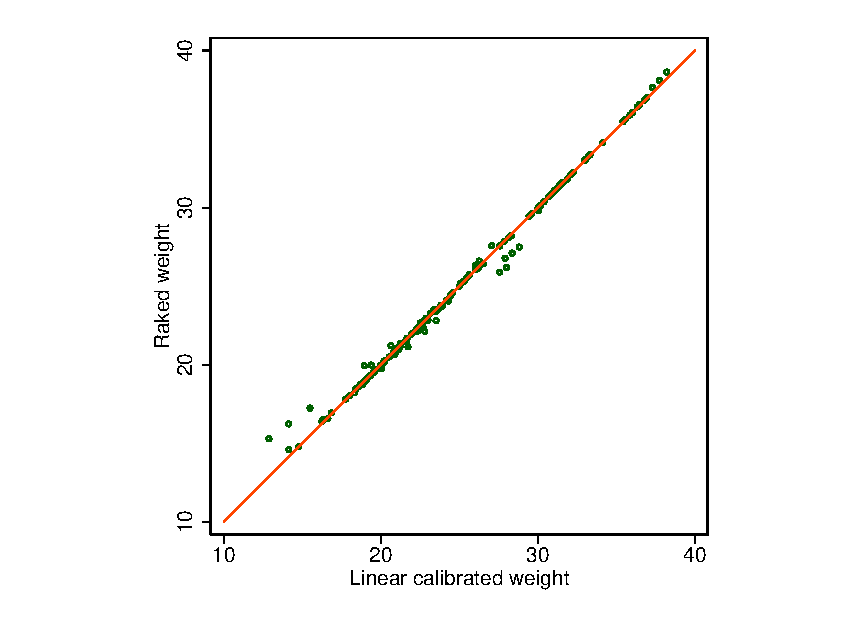
\epsfig{file=raked_linear}
    \end{center}
    \caption{Linear and raked weights}
    \label{fig:linear:raked}
\end{figure}















\subsection{Utility programs}
\label{subsec:utility}

The original package \stcmd{ipfraking} provided two additional utility programs,
\stcmd{mat2do} and \stcmd{xls2row}. An additional utility program was added
to compute the design effects and margins of error, common tasks associated
with describing survey weights. Specifically, the Transparency Initiative
of the American Association for Public Opinion Research
\citep{aapor:2014:ti:terms}
requires that

\begin{quote}
For probability samples, the estimates of sampling error will be reported, and the discussion will state whether or not the reported margins of sampling error or statistical analyses have been adjusted for the design effect due to weighting, clustering, or other factors.
\end{quote}

\begin{stsyntax}
whatsdeff
{\it weight\_variable}
\optif\
\optin\
,
\optional{
by(\varlist)
}
\end{stsyntax}

The utility program \stcmd{whatsdeff} calculates the apparent design effect due to unequal weighting,
${\rm DEFF_{UWE}}=1 + {CV}^2_w = $ \stcmd{1 + r(Var)/(r(mean))\^2} from \stcmd{summarize} {\it weight\_variable}.
Additionally, it reports the effective sample size, $n/{\rm DEFF_{UWE}}$, and also returns
the margins of error for the sample proportions that estimate the population proportions of
10\% and 50\%.

\begin{stlog}
. webuse nhanes2, clear
{\smallskip}
. whatsdeff finalwgt
{\smallskip}
    Group     {\VBAR}   Min     {\VBAR}   Mean    {\VBAR}   Max     {\VBAR}    CV   {\VBAR}   DEFF  {\VBAR}   N   {\VBAR}  N eff
\HLI{14}{\PLUS}\HLI{11}{\PLUS}\HLI{11}{\PLUS}\HLI{11}{\PLUS}\HLI{9}{\PLUS}\HLI{9}{\PLUS}\HLI{7}{\PLUS}\HLI{8}
      Overall {\VBAR}   2000.00 {\VBAR}  11318.47 {\VBAR}  79634.00 {\VBAR}  0.6453 {\VBAR}  1.4164 {\VBAR} 10351 {\VBAR} 7307.97
{\smallskip}
. return list
{\smallskip}
scalars:
                  r(N) =  10351
              r(MOE10) =  .0068792766212984
              r(MOE50) =  .0114654610354974
       r(Neff_Overall) =  7307.97435325364
       r(DEFF_Overall) =  1.416397964696134
{\smallskip}
. whatsdeff finalwgt, by(sex)
{\smallskip}
    Group     {\VBAR}   Min     {\VBAR}   Mean    {\VBAR}   Max     {\VBAR}    CV   {\VBAR}   DEFF  {\VBAR}   N   {\VBAR}  N eff
\HLI{14}{\PLUS}\HLI{11}{\PLUS}\HLI{11}{\PLUS}\HLI{11}{\PLUS}\HLI{9}{\PLUS}\HLI{9}{\PLUS}\HLI{7}{\PLUS}\HLI{8}
sex           {\VBAR}           {\VBAR}           {\VBAR}           {\VBAR}         {\VBAR}         {\VBAR}       {\VBAR}
         Male {\VBAR}   2000.00 {\VBAR}  11426.14 {\VBAR}  79634.00 {\VBAR}  0.6578 {\VBAR}  1.4326 {\VBAR}  4915 {\VBAR} 3430.94
       Female {\VBAR}   2130.00 {\VBAR}  11221.12 {\VBAR}  61534.00 {\VBAR}  0.6333 {\VBAR}  1.4010 {\VBAR}  5436 {\VBAR} 3880.01
\HLI{14}{\PLUS}\HLI{11}{\PLUS}\HLI{11}{\PLUS}\HLI{11}{\PLUS}\HLI{9}{\PLUS}\HLI{9}{\PLUS}\HLI{7}{\PLUS}\HLI{8}
      Overall {\VBAR}   2000.00 {\VBAR}  11318.47 {\VBAR}  79634.00 {\VBAR}  0.6453 {\VBAR}  1.4164 {\VBAR} 10351 {\VBAR} 7307.97
{\smallskip}
. return list
{\smallskip}
scalars:
                  r(N) =  10351
              r(MOE10) =  .0068792766212984
              r(MOE50) =  .0114654610354974
       r(Neff_Overall) =  7307.97435325364
       r(DEFF_Overall) =  1.416397964696134
        r(Neff_Female) =  3880.00710397866
        r(DEFF_Female) =  1.40102836266093
          r(Neff_Male) =  3430.938195872213
          r(DEFF_Male) =  1.432552765279559
{\smallskip}
\nullskip
\end{stlog}

















\clearpage\newpage






















\section{Examples}
\label{sec:examples}

\subsection{Basic syntax and input requirements}
\label{subsec:basic}

In this very simple example, I shall demonstrate the basic mechanics of
\stcmd{ipfraking}, its input requirements and output.
These examples are intended to only demonstrate the syntax
and the output of \stcmd{ipfraking}, and may or may not provide
substantively meaningful results.


\begin{stexample}[Example 1]

We shall work with the standard example of \stcmd{svy} data,
an excerpt from the NHANES II data set available from Stata Corp.\ website.
We shall introduce some small changes to the data so that
\stcmd{ipfraking} will have some work to do.

\begin{stlog}
. webuse nhanes2, clear
{\smallskip}
. generate byte _one = 1
{\smallskip}
.
. svy : total _one , over( sex, nolabel )
(running total on estimation sample)
{\smallskip}
Survey: Total estimation
{\smallskip}
Number of strata =      31       Number of obs    =      10351
Number of PSUs   =      62       Population size  =  117157513
                                 Design df        =         31
{\smallskip}
            1: sex = 1
            2: sex = 2
{\smallskip}
\HLI{13}{\TOPT}\HLI{48}
             {\VBAR}             Linearized
        Over {\VBAR}      Total   Std. Err.     [95\% Conf. Interval]
\HLI{13}{\PLUS}\HLI{48}
_one         {\VBAR}
           1 {\VBAR}   5.62e+07    1377465      5.34e+07    5.90e+07
           2 {\VBAR}   6.10e+07    1396159      5.82e+07    6.38e+07
\HLI{13}{\BOTT}\HLI{48}
{\smallskip}
. matrix NHANES2_sex = e(b)
{\smallskip}
. matrix rownames NHANES2_sex = sex
{\smallskip}
.
{\smallskip}
. svy : total _one , over( race, nolabel )
(running total on estimation sample)
{\smallskip}
Survey: Total estimation
{\smallskip}
Number of strata =      31       Number of obs    =      10351
Number of PSUs   =      62       Population size  =  117157513
                                 Design df        =         31
{\smallskip}
            1: race = 1
            2: race = 2
            3: race = 3
{\smallskip}
\cnp
\HLI{13}{\TOPT}\HLI{48}
             {\VBAR}             Linearized
        Over {\VBAR}      Total   Std. Err.     [95\% Conf. Interval]
\HLI{13}{\PLUS}\HLI{48}
_one         {\VBAR}
           1 {\VBAR}   1.03e+08    2912042      9.71e+07    1.09e+08
           2 {\VBAR}   1.12e+07    1458814       8213964    1.42e+07
           3 {\VBAR}    2968728    1252160      414930.1     5522526
\HLI{13}{\BOTT}\HLI{48}
{\smallskip}
. matrix NHANES2_race = e(b)
{\smallskip}
. matrix rownames NHANES2_race = race
{\smallskip}
.
. matrix NHANES2_sex[1,1] = NHANES2_sex[1,1]*1.25
{\smallskip}
. matrix NHANES2_race[1,1] = NHANES2_race[1,1]*1.4
{\smallskip}
.
\nullskip
\end{stlog}

Let us now look at the matrices that will serve as an input to the
raking procedure.

\begin{stlog}
. matrix list NHANES2_sex, f(\%12.0g)
{\smallskip}
NHANES2_sex[1,2]
         _one:     _one:
            1         2
sex  70199350  60998033
{\smallskip}
. matrix list NHANES2_race, f(\%12.0g)
{\smallskip}
NHANES2_race[1,3]
             _one:        _one:        _one:
                1            2            3
race  144199368.6     11189236      2968728
{\smallskip}
\nullskip
\end{stlog}

These input matrices are organized as follows. Input matrices always
have a single row, just as estimation results \stcmd{e(b)} do. The column
names follow the naming conventions of \stcmd{e(b)}, namely,
the name of the variable for which the total is being computed
(here, \stcmd{\_one}) and the numeric categories of the variable that
was used in the \stcmd{over} option (here, \stcmd{sex}, with values 1 for males
and 2 for females; and \stcmd{race}, with values 1 for whites, 2 for blacks,
and 3 for other). These values must be in an increasing order.
Since that variable is not stored in the e(b) per se,
it needs to be added to this matrix, which is done in the form of the row name.
The entries of the matrix are the totals that the weights in the categories
of the control variables need to sum up to. In this example, they are scaled
to be the population totals. Alternatively, these can be made to sum up to the
sample size, as is done sometimes in public opinion research, or to 1, which
is what \stcmd{proportion} estimation command would produce.

The input requirements in terms of control totals are thus made as simple as possible.
If a higher quality survey is available, all the survey statistician needs to do
is to obtain the totals for the categories of the control variables
using \stcmd{svy: total $\cdots$, over( $\cdots$, nolabel ) }
and save the name of that variable along with the matrix.
Note that the \stcmd{total}
is computed with \stcmd{over( \ldots, nolabel)} suboption to suppress
the otherwise informative labeling of the categories;
\stcmd{ipfraking} expects the numeric values of the categories
as column names (see \pref{matrix rownames}).
The name of the matrix itself is immaterial, but it is
a good programming practice
to have informative names \citep{mcconnell:2004}. Thus the names
of the matrices in the examples generally follow the convention
{\it data{\_}source}{\_}{\it variable}.

We are now ready to run \stcmd{ipfraking} and see what it produces.

\begin{stlog}
. ipfraking [pw=finalwgt], ctotal( NHANES2_sex NHANES2_race ) gen( rakedwgt1 )
{\smallskip}
Warning: the totals of the control matrices are different:
   Target 1 (NHANES2_sex) total              =            131197383
   Target 2 (NHANES2_race) total             =          158357332.6
{\smallskip}
 Iteration 1, max rel difference of raked weights = .56227988
 Iteration 2, max rel difference of raked weights = .00073288
 Iteration 3, max rel difference of raked weights = 2.356e-07
Warning: the controls NHANES2_sex did not match
{\smallskip}
   Summary of the weight changes
{\smallskip}
              {\VBAR}    Mean    Std. dev.    Min        Max       CV
\HLI{14}{\PLUS}\HLI{50} 
Orig weights  {\VBAR}    11318       7304      2000       79634   .6453
Raked weights {\VBAR}    15299      10274      1914       90831   .6716
Adjust factor {\VBAR}   1.3490               0.8846      1.5614
{\smallskip}
\nullskip
\end{stlog}

In this simple case with just two control variables
and the control totals that are not very different from the
existing sample totals, the procedure converged very quickly
in three iterations. A diagnostic message was produced upfront
by \stcmd{ipfraking} informing about apparent differences in
total population counts as obtained from the different
control total matrices. As a result, the control totals
for the variable that was adjusted first (\stcmd{sex})
could not match the required control totals even after the
weights converged in the sense of differing little between
iterations. Both of these warnings are only produced when
problems are encountered.

The summary table is always produced, and shows some relevant
characteristics of the original weights $w_{1j}$, the raked weights
$w_{3j}$, and the raking ratios $w_{3j}/w_{1j}$. As expected,
the coefficient of variation went up from 0.645 to 0.672.

The graphic output produced by \stcmd{ipfraking} is shown on
Figure \ref{fig:example1}. Generally, we would want to inspect these
graphs to see if there any unexpected patterns, such as highly outlying values,
gaps in the distribution (here, there are only six distinct values of the
adjustment factor corresponding to the $2\times3$ combinations of the control
variables) or concentration near the limits of the
weight range (as is typical for trimmed weights, see below in section
\ref{subsec:example:trimming}). Also, these graphs
may inform later trimming decisions: the trimming limits can be
chosen to conform to the breaks in the distributions of
the untrimmed raked weights.

\begin{figure}[h!]
\begin{center}
\epsfig{file=ipfraking_example1}
\end{center}
\caption{Histograms of the raked weights and calibration ratios, Example 1.}
\label{fig:example1}
\end{figure}

\end{stexample}

\subsection{Preparing control matrices from scratch}
\label{subsec:acs}

In many situations, the control totals will be obtained
from outside of Stata, and need to be prepared to work
with \stcmd{ipfraking}.

\begin{stexample}[Example 2]

Suppose I wanted to calibrate
the NHANES II data set to the latest control totals available
from the US Census Bureau website. Using the tables
S0101 from the 2011 American Community Survey 1-year estimates
and NST-EST2011 from the US Census Bureau population projections,
the latest available at the time of writing this paper,
the figures displayed in Table \ref{tab:example2} can be obtained.

\begin{table}
\caption{Control totals for the 2011 US population.\label{tab:example2}}

\centering

\begin{tabular}{p{5cm}l}
    Group & Population \\
    \hline
    \multicolumn{2}{c}{~~ACS 2011 1-year estimates, Table S0101~~} \\
    Male, total & 153,267,860 \\
    Ages 20--39 & 27.4\% \\
    Ages 40--59 & 27.5\% \\
    Ages 60+    & 17.3\% \\
    Female, total & 158,324,057 \\
    Ages 20--39 & 26.0\% \\
    Ages 40--59 & 27.6\% \\
    Ages 60+    & 20.7\% \\
    \multicolumn{2}{c}{~~US Census Bureau 2011 projections, Table NST-EST2011-01~~} \\
    Northeast & 55,521,598 \\
    Midwest   & 67,158,835 \\
    South     & 116,046,736 \\
    West      & 72,864,748 \\
    \multicolumn{2}{c}{~~US Census Bureau 2011 projections, Table NC-EST2011-03~~} \\
    White     & 243,470,497 \\
    Black     & 40,750,746 \\
    Other     & 27,370,674 \\
    \hline
    Total     & 311,591,917
\end{tabular}
\end{table}

Thus, we have information in the two-way age by sex table, as well
as two additional margins. We shall need an additional sex-by-age group variable,
and we shall try to make its values somewhat informative
(e.g., the value \stcmd{12} of the variable \stcmd{sex\_age} means
the first group of sex and the second group of age):

\begin{stlog}
. generate byte age_grp = 1 + (age>=40) + (age>=60) if !mi(age)
{\smallskip}
. generate sex_age = sex*10 + age_grp
{\smallskip}
\nullskip
\end{stlog}

With that, the matrices will have to be defined explicitly,
and their labels need to be hand-coded, too (see \pref{matrix rownames}).
Note that the US Census Bureau 2011
projections relate to the total population, while the target population
of the study is the population age 20+. Assuming that the age structure
is the same across regions and races, the control totals for region and race
need to be rescaled to the adult population to avoid the warning messages.
(More accurate figures can be obtained from ACS microdata which can be downloaded
from the U.S.\ Census Bureau website.)

\begin{stlog}
. matrix ACS2011_sex_age = ( ///
>     153267860*0.274, 153267860*0.275, 153267860*0.173, /// males
>     158324057*0.260, 158324057*0.276, 158324057*0.207  /// females
> )
{\smallskip}
. matrix colnames ACS2011_sex_age = 11 12 13 21 22 23
{\smallskip}
. matrix coleq    ACS2011_sex_age = _one
{\smallskip}
. matrix rownames ACS2011_sex_age = sex_age
{\smallskip}
. scalar ACS2011_total_pop = 311591917
{\smallskip}
. matrix ACS2011_adult_pop = ACS2011_sex_age * J(colsof(ACS2011_sex_age),1,1)
{\smallskip}
. matrix Census2011_region = ///
>     (55521598, 67158835, 116046736, 72864748 )
{\smallskip}
. matrix Census2011_region = Census2011_region * ACS2011_adult_pop / ACS2011_to
> tal_pop
{\smallskip}
. matrix colnames Census2011_region = 1 2 3 4
{\smallskip}
. matrix coleq    Census2011_region = _one
{\smallskip}
. matrix rownames Census2011_region = region
{\smallskip}
. matrix Census2011_race = ///
>     (243470497, 40750746, 27370674 )
{\smallskip}
\cnp
. matrix Census2011_race = Census2011_race * ACS2011_adult_pop / ACS2011_total_
> pop
{\smallskip}
. matrix colnames Census2011_race = 1 2 3
{\smallskip}
. matrix coleq    Census2011_race = _one
{\smallskip}
. matrix rownames Census2011_race = race
{\smallskip}
\nullskip
\end{stlog}

Let us check the matrix entries and labels once again before
producing the weights.
Note that the values of the control variable categories are given in an increasing order.

\begin{stlog}
. matrix list ACS2011_sex_age, f(\%10.0g)
{\smallskip}
ACS2011_sex_age[1,6]
             _one:     _one:     _one:     _one:     _one:     _one:
               11        12        13        21        22        23
sex_age  41995394  42148662  26515340  41164255  43697440  32773080
{\smallskip}
. matrix list Census2011_region, f(\%10.0g)
{\smallskip}
Census2011_region[1,4]
            _one:     _one:     _one:     _one:
               1         2         3         4
region  40679030  49205289  85024007  53385843
{\smallskip}
. matrix list Census2011_race, f(\%11.0g)
{\smallskip}
Census2011_race[1,3]
            _one:       _one:       _one:
               1           2           3
race   178383622  29856864.7  20053682.2
{\smallskip}
\nullskip
\end{stlog}

As the labels appear to be in place, let us run \stcmd{ipfraking}:

\begin{stlog}
. ipfraking [pw=finalwgt], gen( rakedwgt2 ) ///
>     ctotal( ACS2011_sex_age Census2011_region Census2011_race ) 
{\smallskip}
 Iteration 1, max rel difference of raked weights = 14.95826
 Iteration 2, max rel difference of raked weights = .19495004
 Iteration 3, max rel difference of raked weights = .02204455
 Iteration 4, max rel difference of raked weights = .00315355
 Iteration 5, max rel difference of raked weights = .00043857
 Iteration 6, max rel difference of raked weights = .00006061
 Iteration 7, max rel difference of raked weights = 8.365e-06
 Iteration 8, max rel difference of raked weights = 1.154e-06
 Iteration 9, max rel difference of raked weights = 1.593e-07
{\smallskip}
   Summary of the weight changes
{\smallskip}
              {\VBAR}    Mean    Std. dev.    Min        Max       CV
\HLI{14}{\PLUS}\HLI{50} 
Orig weights  {\VBAR}    11318       7304      2000       79634   .6453
Raked weights {\VBAR}    22055      19227      4050      338675   .8717
Adjust factor {\VBAR}   2.1464               0.9264     18.3694
{\smallskip}
\nullskip
\end{stlog}

The diagnostic plots for these weights are given in Figure \ref{fig:example2}.
They do appear to have some outlying cases (which are not very clearly seen
on these plots as they are single count observations with outlying weights),
and we shall address them in the next section with trimming.

\begin{figure}[h!]
\begin{center}
\epsfig{file=ipfraking_example2}
\end{center}
\caption{Histograms of the raked weights and calibration ratios, Example 2.}
\label{fig:example2}
\end{figure}

\end{stexample}

\subsection{Trimming options}
\label{subsec:example:trimming}


As discussed in Section \ref{subsec:trimming} above, if variability of the weights
becomes excessive, the weights can be trimmed by restricting the extremes.
Using \stcmd{ipfraking} options, upper and/or lower limits can be defined
for either the absolute values of the weights or the relative changes from
the base weights. The frequency of the trimming operations can also be controlled.
Trimming can be applied once to the final data (\stcmd{trimfreq(once)})
at step \ref{step:trimfreq:once} of Algorithm 2.
Alternatively, trimming can be applied after every full cycle over variables
at step \ref{step:trimfreq:sometimes} of Algorithm 2.
Finally, trimming can be applied after each sub-iteration
at step \ref{step:trimfreq:often} of the algorithm.

\begin{stexample}[Example 3]

Inspecting the histograms on Figure \ref{fig:example2}, it appears reasonable
to restrict the upper tail of the raked weights. A more detailed investigation
of the histogram reveals a somewhat greater concentration of the raked weights
around the value of 160,000, and sparse bars beyond 200,000. This latter number
will be used as the top cut-off point for trimming, and is provided as an input
to \stcmd{ipfraking} via option \stcmd{trimhiabs}. Also, I specified the absolute
lower bound of 2,000, which is the minimum of the original weights, but,
as the output in the previous example suggested, the calibrated weights tend to run
above 4,000, so specifying the lower limit as \stcmd{trimloabs(2000)} may not really
affect the calibration procedure.

\begin{stlog}
. ipfraking [pw=finalwgt], gen( rakedwgt3 ) ///
>     ctotal( ACS2011_sex_age Census2011_region Census2011_race ) ///
>     trimhiabs( 200000 ) trimloabs( 2000 )
{\smallskip}
 Iteration 1, max rel difference of raked weights = 14.95826
 Iteration 2, max rel difference of raked weights = .21474256
 Iteration 3, max rel difference of raked weights = .02754514
 Iteration 4, max rel difference of raked weights = .00511347
 Iteration 5, max rel difference of raked weights = .00095888
 Iteration 6, max rel difference of raked weights = .00018036
 Iteration 7, max rel difference of raked weights = .00003391
 Iteration 8, max rel difference of raked weights = 6.377e-06
 Iteration 9, max rel difference of raked weights = 1.199e-06
 Iteration 10, max rel difference of raked weights = 2.254e-07
{\smallskip}
   Summary of the weight changes
{\smallskip}
              {\VBAR}    Mean    Std. dev.    Min        Max       CV
\HLI{14}{\PLUS}\HLI{50} 
Orig weights  {\VBAR}    11318       7304      2000       79634   .6453
Raked weights {\VBAR}    22055      18908      4033      200000   .8573
Adjust factor {\VBAR}   2.1486               0.9220     18.9828
{\smallskip}
\nullskip
\end{stlog}

The resulting coefficient of variation of weights, 0.857, is slightly
better than that with unrestricted range of weights, 0.872. The summary also shows
that the weights were capped at 200,000, as requested.

Setting the absolute limits on the range of the raked weights is often
very subjective. A somewhat better plan might be to set limits in terms
of the range of the adjustment factors, as shown in the next example. The relative
change in the weights can be bounded with \stcmd{trimlorel()} and \stcmd{trimhirel()}
options.
I also demonstrate here how to use the results of \stcmd{summarize} to feed
into \stcmd{ipfraking}. While ensuring that accurate numbers are being carried
over in the context of the code, the approach is fragile for interactive
work: simply running the single line with the sole
\stcmd{ipfraking} command that refers to the \stcmd{r()} return values
may break down if \stcmd{summarize} was not the
immediately preceding command.

\begin{stlog}
. sum finalwgt
{\smallskip}
    Variable {\VBAR}       Obs        Mean    Std. Dev.       Min        Max
\HLI{13}{\PLUS}\HLI{56}
    finalwgt {\VBAR}     10351    11318.47     7304.04       2000      79634
{\smallskip}
. ipfraking [pw=finalwgt], gen( rakedwgt4 ) ///
>     ctotal( ACS2011_sex_age Census2011_region Census2011_race ) ///
>     trimhiabs(`=2.5*r(max)') trimloabs(`=r(min)') trimhirel(6)
{\smallskip}
\cnp
 Iteration 1, max rel difference of raked weights = 5
 Iteration 2, max rel difference of raked weights = .25592859
 Iteration 3, max rel difference of raked weights = .0626759
 Iteration 4, max rel difference of raked weights = .0158786
 Iteration 5, max rel difference of raked weights = .00299304
 Iteration 6, max rel difference of raked weights = .00070812
 Iteration 7, max rel difference of raked weights = .00016401
 Iteration 8, max rel difference of raked weights = .00003734
 Iteration 9, max rel difference of raked weights = 8.434e-06
 Iteration 10, max rel difference of raked weights = 1.898e-06
 Iteration 11, max rel difference of raked weights = 4.265e-07
Warning: the controls ACS2011_sex_age did not match
Warning: the controls Census2011_region did not match
Warning: the controls Census2011_race did not match
{\smallskip}
   Summary of the weight changes
{\smallskip}
              {\VBAR}    Mean    Std. dev.    Min        Max       CV
\HLI{14}{\PLUS}\HLI{50}
Orig weights  {\VBAR}    11318       7304      2000       79634   .6453
Raked weights {\VBAR}    21830      18115      4113      199085   .8298
Adjust factor {\VBAR}   2.1323               0.8973      6.0000
{\smallskip}
\nullskip
\end{stlog}

\end{stexample}

Setting the trimming options too aggressively may lead to adverse
consequences. First, it may bias the estimates, as discussed in Section
\ref{subsec:pro:con}.
Second, as this example demonstrates, it can impede (statistical) convergence:
the output contains multiple warnings about targets not being achieved
within desired accuracy, while no problems were encountered without trimming.

\subsection{Tracking convergence}
\label{subsec:example:trace}

Let us now look in more detail into the issue of trimming frequency,
and demonstrate another diagnostic plot that can be produced by
\stcmd{ipfraking}.

\begin{stexample}[Example 4]

We return to the first set of options of Example 3, and
re-run the raking procedure.

\begin{stlog}
. capture drop rakedwgt3
{\smallskip}
. ipfraking [pw=finalwgt], gen( rakedwgt3 ) ///
>     ctotal( ACS2011_sex_age Census2011_region Census2011_race ) ///
>     trimhiabs(200000) trimloabs(2000) trimfreq(sometimes) trace
{\smallskip}
 Iteration 1, max rel difference of raked weights = 14.95826
\oom
 Iteration 10, max rel difference of raked weights = 2.254e-07
{\smallskip}
   Summary of the weight changes
{\smallskip}
              {\VBAR}    Mean    Std. dev.    Min        Max       CV
\HLI{14}{\PLUS}\HLI{50}
Orig weights  {\VBAR}    11318       7304      2000       79634   .6453
Raked weights {\VBAR}    22055      18908      4033      200000   .8573
Adjust factor {\VBAR}   2.1486               0.9220     18.9828
{\smallskip}
\nullskip
\end{stlog}

The option \stcmd{trace} requests that trace plots be added to
the diagnostic plots, as shown on Figure \ref{fig:example4:sometimes}.
The trace plots are presented on the absolute scale and on the log scale.
The exponentially declining discrepancy appears to be a general phenomenon.
In other words, after the first few iterations,
discrepancy between the currently weighted totals to the control totals roughly follows
the rate of $\rm{const} \times \alpha^k$ for some $\alpha<1$, where $k$ is
the (outer cycle) iteration number. When convergence is very slow or the sample
size is very large, this rule may be helpful in determining the number
of iterations necessary to achieve the required accuracy, and hence
the expected computing time. Zero cross-cells and collinearity between
the control variables may make the convergence factor $\alpha$ close to 1 thus
hampering convergence. This happens when the control variables have
very similar meaning, such as age and grade of children: it is impossible
to have children of age 8 in grade 10.
Also, sets of interactions of categorical variables, such as interactions
of age group and education along with age group and race, are guaranteed to
produce zero cells in the cross-tabulation: it is impossible to have
any observations in the cells defined say by
(age under 40 interacted with higher education) on one margin against
(age above 60 interacted with white race) on the other.

\begin{figure}[!th]
\begin{center}
\epsfig{file=ipfraking_example4_sometimes}
\end{center}
\caption{Diagnostic plots for Example 4.}
\label{fig:example4:sometimes}
\end{figure}

While \stcmd{trimfreq(sometimes)} is the default in presence
of other trimming options, the behavior can be changed
with explicit specification of trimming frequency. Note that slightly
different weights will be produced that way.

\begin{stlog}
. ipfraking [pw=finalwgt], gen( rakedwgt5 ) ///
>     ctotal( ACS2011_sex_age Census2011_region Census2011_race ) ///
>     trimhiabs(200000) trimloabs(2000) trimfreq(often) trace
{\smallskip}
\cnp
 Iteration 1, max rel difference of raked weights = 14.95826
 Iteration 2, max rel difference of raked weights = .21613885
 Iteration 3, max rel difference of raked weights = .02673316
 Iteration 4, max rel difference of raked weights = .00480164
 Iteration 5, max rel difference of raked weights = .00086195
 Iteration 6, max rel difference of raked weights = .00015444
 Iteration 7, max rel difference of raked weights = .00002762
 Iteration 8, max rel difference of raked weights = 4.940e-06
 Iteration 9, max rel difference of raked weights = 8.832e-07
{\smallskip}
   Summary of the weight changes
{\smallskip}
              {\VBAR}    Mean    Std. dev.    Min        Max       CV
\HLI{14}{\PLUS}\HLI{50}
Orig weights  {\VBAR}    11318       7304      2000       79634   .6453
Raked weights {\VBAR}    22055      18905      4033      200000   .8572
Adjust factor {\VBAR}   2.1487               0.9220     18.9844
{\smallskip}
. compare rakedwgt3 rakedwgt5
{\smallskip}
                                        \HLI{10} difference \HLI{10}
                            count       minimum      average     maximum
\HLI{72}
rakedwgt3<rakedwgt5          3638     -15.27963    -1.226753   -.0128687
rakedwgt3=rakedwgt5             4
rakedwgt3>rakedwgt5          6709      .0011514     .6652557    2471.578
                       \HLI{10}
jointly defined             10351     -15.27963     .0000264    2471.578
                       \HLI{10}
total                       10351
{\smallskip}
\nullskip
\end{stlog}

In this example, trimming the weights after adjusting each of the margins
led to fewer iterations. This may or may not translate to lower overall
computing times as more computing is performed within each iteration.

\end{stexample}

\subsection{Metadata}
\label{subsec:example:meta}

The results of raking operations can be stored with the newly created
weight variables for later review and reproduction of the results.
Let us reproduce the example in the previous section adding all the metadata
available:

\begin{stexample}[Example 5]

\begin{stlog}
. capture drop rakedwgt3
{\smallskip}
. ipfraking [pw=finalwgt], gen( rakedwgt3 ) ///
>     ctotal( ACS2011_sex_age Census2011_region Census2011_race ) ///
>     trimhiabs(200000) trimloabs(2000) meta
{\smallskip}
\cnp
 Iteration 1, max rel difference of raked weights = 14.95826
\oom
 Iteration 10, max rel difference of raked weights = 2.254e-07
{\smallskip}
   Summary of the weight changes
{\smallskip}
              {\VBAR}    Mean    Std. dev.    Min        Max       CV
\HLI{14}{\PLUS}\HLI{50}
Orig weights  {\VBAR}    11318       7304      2000       79634   .6453
Raked weights {\VBAR}    22055      18908      4033      200000   .8573
Adjust factor {\VBAR}   2.1486               0.9220     18.9828
{\smallskip}
. char li rakedwgt3[]
  rakedwgt3[command]:         [pw=finalwgt], gen( rakedwgt3 ) ctotal( ACS2011_s
> ex_age Ce..
  rakedwgt3[trimloabs]:       trimloabs(2000)
  rakedwgt3[trimhiabs]:       trimhiabs(200000)
  rakedwgt3[trimfrequency]:   sometimes
  rakedwgt3[objfcn]:          2.25435521346e-07
  rakedwgt3[maxctrl]:         3.00266822363e-08
  rakedwgt3[converged]:       1
  rakedwgt3[Census2011_race]: 7.48567503861e-09
  rakedwgt3[Census2011_region]:
                              3.00266822363e-08
  rakedwgt3[ACS2011_sex_age]: 4.13778410340e-09
  rakedwgt3[note1]:           Raking controls used: ACS2011_sex_age Census2011_
> region Ce..
  rakedwgt3[note0]:           1
{\smallskip}
\nullskip
\end{stlog}

\end{stexample}

The following characteristics are stored with the newly created weight variable
(see \pref{char}).

\begin{tabular}{ll}
    \stcmd{command} & The full command as typed by the user \\
    {\it matrix name} & The relative matrix difference from the corresponding \\
                    & control total, see \dref{functions} \\
    \stcmd{trimhiabs}, \stcmd{trimloabs}, & Corresponding trimming options,
                    if specified \\
    \stcmd{trimhirel}, \stcmd{trimlorel}, & \\
    \stcmd{trimfrequency} & \\
    \stcmd{maxctrl} & the greatest \stcmd{mreldif} between the targets \\
                    & and the achieved weighted totals \\
    \stcmd{objfcn}  & the value of the relative weight change $D_k$ (\ref{eq:conv:ratio:weights})
                    at exit \\
    \stcmd{converged} & whether \stcmd{ipfraking} exited due to convergence (1) \\
                    & vs. due to an increase in the objective function \\
                    & or reaching the limit on the number of iterations (0)
\end{tabular}

Also, \stcmd{ipfraking} stores the notes regarding the control matrices
used, and which of the margins did not match the control totals, if any.
See \dref{notes}.

\subsection{Replicate weights}

As discussed in Section \ref{subsec:variance}, one of the greater challenges
of weight calibration is ensuring that variance estimates take into account
the greater precision achieved by adjusting the sample towards the fixed
population quantities. As estimating the variances using linearization
is cumbersome, replicate variance estimation may be more attractive.

\begin{stexample}[Example 6]

The simplest code for calibrated replicate weights is obtained by calling
\stcmd{ipfraking} from within \stcmd{bsweights} \citep{kolenikov:2010}
which can pass the name of a replicate weight variable to an arbitrary
calibration routine. In this example, we shall use the same settings
as in Section \ref{subsec:acs} and thus we shall have the calibrated weight
\stcmd{rakedwgt2} which was produced in that example as the main weight
for which the bootstrap weights provide the measure of sampling variability.

\begin{stlog}
. set seed 2013
{\smallskip}
. set rmsg on
r; t=0.00 14:50:44
{\smallskip}
. bsweights bsw , reps(310) n(-1) balanced dots ///
>     calibrate( ipfraking [pw=@], replace nograph meta ///
>     ctotal( ACS2011_sex_age Census2011_region Census2011_race ) )
Balancing within strata:
...............................
{\smallskip}
Rescaling weights
..................................................    50
..................................................   100
..................................................   150
..................................................   200
..................................................   250
..................................................   300
..........
{\smallskip}
r; t=178.79 14:53:43
{\smallskip}
. forvalues k=1/310 {\lbr}
  2.     _dots `k' 0
  3.     assert `: char bsw`k'[converged]' == 1
  4.     assert `: char bsw`k'[maxctrl]' < 10*c(epsfloat)
  5. {\rbr}
..................................................    50
..................................................   100
..................................................   150
..................................................   200
..................................................   250
..................................................   300
..........r; t=0.32 14:53:43
{\smallskip}
. set rmsg off
{\smallskip}
. svyset [pw=rakedwgt2], vce(bootstrap) bsrw( bsw* ) dof( 31 )
{\smallskip}
      pweight: rakedwgt2
          VCE: bootstrap
          MSE: off
    bsrweight: bsw1 bsw2 bsw3 bsw4 bsw5 bsw6 bsw7 bsw8 bsw9 bsw10 bsw11 bsw12
\oom
               bsw301 bsw302 bsw303 bsw304 bsw305 bsw306 bsw307 bsw308 bsw309
               bsw310
    Design df: 31
  Single unit: missing
     Strata 1: <one>
         SU 1: <observations>
        FPC 1: <zero>
{\smallskip}
\nullskip
\end{stlog}

The options of \stcmd{bsweights} request 310 replicate weights
(a multiple of 31 strata), resample one less PSU than available in
a given stratum, and obtain the first-order balance within a stratum.
With the 2 PSU/stratum design and these options, \stcmd{bsweights}
produces random half-samples of data. The at-character \stcmd{@} is a placeholder
for the name of the replicate weight variable.
For explanations of these and other options of \stcmd{bsweights},
see \citet{kolenikov:2010}. The procedure took about 3 minutes
on a laptop computer, which can be considered moderately
computationally intensive beyond interactive.
A new option of \stcmd{ipfraking} in the above code is
\stcmd{nograph} that suppresses the histograms.
The additional asserts \citep{gould:2003:tip3} following the bootstrap
weight generation demonstrate how the minimal quality assurance
can be done on the bootstrap weights in the weight production workflow.


A more compact set of weights can be developed based on the existing
BRR weights and a slightly more explicit code cycling over the weight
variables:

\begin{stlog}
. webuse nhanes2brr, clear
{\smallskip}
. svy : proportion highbp
(running proportion on estimation sample)
{\smallskip}
BRR replications (32)
\HLI{4}{\PLUS}\HLI{3} 1 \HLI{3}{\PLUS}\HLI{3} 2 \HLI{3}{\PLUS}\HLI{3} 3 \HLI{3}{\PLUS}\HLI{3} 4 \HLI{3}{\PLUS}\HLI{3} 5
................................
{\smallskip}
Survey: Proportion estimation    Number of obs    =      10351
                                 Population size  =  117157513
                                 Replications     =         32
                                 Design df        =         31
{\smallskip}
\HLI{13}{\TOPT}\HLI{48}
             {\VBAR}                 BRR
             {\VBAR} Proportion   Std. Err.     [95\% Conf. Interval]
\HLI{13}{\PLUS}\HLI{48}
highbp       {\VBAR}
           0 {\VBAR}   .8941859   .0067023      .8805165    .9078553
           1 {\VBAR}   .1058141   .0067023      .0921447    .1194835
\HLI{13}{\BOTT}\HLI{48}
{\smallskip}
. generate byte _one = 1
{\smallskip}
. generate byte age_grp = 1 + (age>=40) + (age>=60) if !mi(age)
{\smallskip}
. generate sex_age = sex*10 + age_grp
{\smallskip}
. ipfraking [pw=finalwgt], gen( rakedwgt2 ) ///
>     ctotal( ACS2011_sex_age Census2011_region Census2011_race )
{\smallskip}
 Iteration 1, max rel difference of raked weights = 14.95826
 Iteration 2, max rel difference of raked weights = .19495004
 Iteration 3, max rel difference of raked weights = .02204455
 Iteration 4, max rel difference of raked weights = .00315355
 Iteration 5, max rel difference of raked weights = .00043857
 Iteration 6, max rel difference of raked weights = .00006061
 Iteration 7, max rel difference of raked weights = 8.365e-06
 Iteration 8, max rel difference of raked weights = 1.154e-06
 Iteration 9, max rel difference of raked weights = 1.593e-07
{\smallskip}
\cnp
   Summary of the weight changes
{\smallskip}
              {\VBAR}    Mean    Std. dev.    Min        Max       CV
\HLI{14}{\PLUS}\HLI{50}
Orig weights  {\VBAR}    11318       7304      2000       79634   .6453
Raked weights {\VBAR}    22055      19227      4050      338675   .8717
Adjust factor {\VBAR}   2.1464               0.9264     18.3694
{\smallskip}
. forvalues k=1/32 {\lbr}
  2.     quietly ipfraking [pw=brr_`k'], gen( brrc_`k' ) nograph ///
>         ctotal( ACS2011_sex_age Census2011_region Census2011_race )
  3.     _dots `k' 0
  4. {\rbr}
................................
. svyset [pw=rakedwgt2], vce(brr) brrw( brrc* ) dof( 31 )
{\smallskip}
      pweight: rakedwgt2
          VCE: brr
          MSE: off
    brrweight: brrc_1 brrc_2 brrc_3 brrc_4 brrc_5 brrc_6 brrc_7 brrc_8 brrc_9
               brrc_10 brrc_11 brrc_12 brrc_13 brrc_14 brrc_15 brrc_16
               brrc_17 brrc_18 brrc_19 brrc_20 brrc_21 brrc_22 brrc_23
               brrc_24 brrc_25 brrc_26 brrc_27 brrc_28 brrc_29 brrc_30
               brrc_31 brrc_32
    Design df: 31
  Single unit: missing
     Strata 1: <one>
         SU 1: <observations>
        FPC 1: <zero>
{\smallskip}
. svy : proportion highbp
(running proportion on estimation sample)
{\smallskip}
BRR replications (32)
\HLI{4}{\PLUS}\HLI{3} 1 \HLI{3}{\PLUS}\HLI{3} 2 \HLI{3}{\PLUS}\HLI{3} 3 \HLI{3}{\PLUS}\HLI{3} 4 \HLI{3}{\PLUS}\HLI{3} 5
................................
{\smallskip}
Survey: Proportion estimation    Number of obs    =      10351
                                 Population size  =  228294169
                                 Replications     =         32
                                 Design df        =         31
{\smallskip}
\HLI{13}{\TOPT}\HLI{48}
             {\VBAR}                 BRR
             {\VBAR} Proportion   Std. Err.     [95\% Conf. Interval]
\HLI{13}{\PLUS}\HLI{48}
highbp       {\VBAR}
           0 {\VBAR}   .8730544   .0081501      .8564323    .8896766
           1 {\VBAR}   .1269456   .0081501      .1103234    .1435677
\HLI{13}{\BOTT}\HLI{48}
\nullskip
\end{stlog}

The data can be analyzed with the standard \stcmd{svy} prefix,
and the standard errors will appropriately capture the efficiency
gains from weight calibration. No additional action is required
for the analyst or researcher.

\end{stexample}

{\bf CAUTION:} the input weights for the replicate weight calibration
must be the probability replicate weights. The existing NHANES II weights
have been adjusted for non-response and calibrated by the data provider,
and are used above for demonstration purposes only.

\section{Error messages and troubleshooting}
\label{subsec:tbshooting}

\subsection{Critical errors}

The following critical errors will stop execution of
\stcmd{ipfraking}.

\noindent
{\tt pweight is required}

\morehang
    The \stcmd{[pweight=\ldots]} component of \stcmd{ipfraking}
    syntax is required. Probability weights must be specified as
    inputs to \stcmd{ipfraking}.

\noindent
    {\tt ctotal() is required}

    \morehang
    The \stcmd{ctotal()} component of \stcmd{ipfraking}
    syntax is required. Names of the matrices containing the
    control totals must be specified.

    \noindent
    {\tt one and only one of generate() or replace must be specified}

    \morehang
    Either \stcmd{generate()} option with the name of the new variable
    must be supplied to \stcmd{ipfraking}, or \stcmd{replace} to replace
    the variable specified in \stcmd{[pw=\ldots]} statement.

    \noindent
    {\tt raking procedure appears diverging}

    \morehang
    The maximum relative difference of weights $D_k$ has increased from
    the previous
    iteration. This may or may not indicate a problem. Re-run \stcmd{ipfraking}
    with \stcmd{nodivergence} option to override the warning.

    \noindent
    {\tt cannot process matrix {\it matrix{\_}name}}

    \morehang
    For whatever reason, \stcmd{ipfraking} could not process this matrix.
    The matrix may not have been defined or the variables in this matrix
    cannot be found.

    \noindent
    {\tt variable {\it varname} corresponding to the control matrix
    {\it matrix{\_}name} \\ not found}

    \morehang
    The variables contained in row or column names of this matrix
    cannot be found.

    \noindent
    {\tt {\it varname1} and {\it varname2} variables are not compatible}

    \morehang
    When running \stcmd{total} {\it varname1}\stcmd{, over(}{\it varname2}\stcmd{)},
    an error was encountered. One of the variables may be a string variable
    or have missing values resulting in an empty estimation sample.

    \noindent
    {\tt categories of {\it varname} do not match in the control {\it matrix{\_}name} \\
    and in the data (nolab option)}

    \morehang
    There was a mismatch in the categories of {\it varname} found in the data
    and in the control matrix {\it matrix{\_}name}. This could happen for any of the
    following reasons: (i) there were more categories in one than in the other;
    (ii) the entries are in the wrong order in the control matrix; (iii) the labels
    in the control matrix do not correspond to the category values in the data set;
    (iv) the control matrix was obtained via \stcmd{total}
    {\it varname2}\stcmd{, over(}{\it varname}\stcmd{)}, but \stcmd{nolabel} suboption
    of \stcmd{over()} was omitted, and the labels of the control matrix may include
    some unexpected text. Tabulate {\it varname} without labels, and compare the results
    to the matrix listing of the {\it matrix{\_}name}.

    \noindent
    {\tt cannot compute controls for {\it matrix{\_}name} over
    {\it varname} with the current \\ weights}

    \morehang
    This is a generic error message that something bad happened while
    \stcmd{ipfraking} was computing the totals for the current set of weights.
    This error message should generally be very rare, but as computing
    the totals may be the slowest operation of the iterative optimization
    process, stopping \stcmd{ipfraking} with a {\it Ctrl+Break} combination or
    the {\it Break} GUI button may produce this error message.

    \noindent
    {\tt trimhiabs|trimloabs|trimhirel|trimlorel must be a positive number}

    \morehang
    One or more of the trimming options are given as a non-positive number
    or a non-number.

    \noindent
    {\tt trimhiabs must be greater than trimloabs}

    \noindent
    {\tt trimhirel must be greater than trimlorel}

    \morehang
    The trimming parameters are illogical (the lower bound is greater than the upper bound).
    Respecify the values of the trimming parameters.

\bigskip

\subsection{Other errors and warnings}

The following warning messages may be produced by
\stcmd{ipfraking}. The program will continue running, but you must
double-check the results for potential problems.

\noindent
    {\tt the totals of the control matrices are different}

    \morehang
    The sum of values of the control matrices are different.
    These sums will be listed for review. Convergence is still
    possible, but some of the control total checks are likely to fail.

    \noindent
    {\tt trimfrequency() option is specified without numeric settings; will be \\ ignored}

    \morehang
    The option \stcmd{trimfrequency()} was specified without any numeric trimming options.
    There is no way to interpret this, and \stcmd{ipfraking} will proceed without
    trimming.

    \noindent
    {\tt trimfrequency() option is specified incorrectly, assume default value \\ (sometimes)}

    \morehang
    Something other than \stcmd{often}, \stcmd{sometimes} or \stcmd{once} was supplied
    in \stcmd{trimfrequency}, and the default value is being used instead.

    \noindent
    {\tt raking procedure did not converge}

    \morehang
    The maximum number of iterations was reached, but weights never met the convergence
    criteria (see step \ref{step:check:weight:conv} of Algorithm 2 in Section \ref{subsec:trimming}).
    The user may want to increase the number of iterations or relax convergence criteria.

    \noindent
    {\tt the controls {\it matrix{\_}name} did not match}

    \morehang
    After convergence of weights was declared, \stcmd{ipfraking}
    checked again the control totals, and found that the results
    differed from the target for one or more of the control total
    matrices. Any of the following can cause this: (i) the sum of
    entries of this particular matrix differs from the others;
    (ii) the trimming options are too restrictive, and do not allow
    the weights to adjust enough; (iii) the problem may not have a
    solution due to incompatible control totals or a bad sample.

    \noindent
    {\tt division by zero weighted total encountered with
    {\it matrix{\_}name} control}

    \morehang
    The weights for a category of the control variable summed
    to zero. \stcmd{ipfraking} will skip calibration over this
    variable and proceed to the next one.

    \noindent
    {\tt \# missing values of {\it varname} encountered; convergence will be impaired}

    \morehang
    A control variable has missing values in the calibration sample.
    There is little way for \stcmd{ipfraking} to figure out how to deal
    with the weights for the observations with missing values. The user would need
    either to restrict the sample to non-missing values of all control variables,
    to impute the missing values or to create a separate category for the missing
    values of a given control variable (which may lead to difficulties in defining
    valid population control totals for it).

\section*{Acknowledgements}

The author is grateful to Ben Phillips, Andrew Burkey and Brady West,
as well as the editor and an anonymous referee,
who suggested additional functionality and provided helpful comments
to improve the readability of this article. The opinions stated in this paper
are of the author only, and do not represent the position of Abt Associates.

\bibliographystyle{sj}
\bibliography{everything}
% \bibliography{ipfraking}

\begin{aboutauthor}
  Stanislav (Stas) Kolenikov is a Senior Scientist at Abt Associates.
  His work involves applications of statistical methods in data collection
  for public opinion research, public health, transportation, and other disciplines
  that utilize collection of survey data.
  Within survey methodology, his expertise includes advanced sampling techniques,
  survey weighting, calibration, missing data imputation, variance estimation,
  nonresponse analysis and adjustment, and small area estimation.
  Besides survey statistics, Stas has extensive experience developing and applying
  statistical methods in social sciences, with focus on structural equation
  modeling and microeconometrics. He has been writing Stata programs since
  1998 when Stata was version 5.
\end{aboutauthor}
